\documentclass[preprint,review,number]{elsarticle}

\usepackage{amsmath,amssymb}
\usepackage{booktabs}
\usepackage{multirow}
\usepackage{graphicx}
\usepackage{algorithm}
\usepackage{algpseudocode}
\usepackage{hyperref}
\usepackage{xcolor}
\usepackage{subcaption}
\usepackage{tikz}
\usepackage{pgfplots}
\pgfplotsset{compat=1.18}
\usepgfplotslibrary{groupplots}
\usetikzlibrary{positioning, arrows.meta, calc, shapes.geometric, fit, backgrounds, patterns}

\bibliographystyle{elsarticle-num}

% Custom commands
\newcommand{\ours}{\textsc{TARA}}
\newcommand{\ie}{\textit{i.e.}}
\newcommand{\eg}{\textit{e.g.}}
\newcommand{\cf}{\textit{cf.}}
\newcommand{\etal}{\textit{et al.}}

\journal{Knowledge-Based Systems}

\begin{document}

\begin{frontmatter}

\title{TARA: Complexity-Adaptive Retrieval Refinement through Tool-Augmented ReAct Agents}

\author[1]{Ruo Lee}
\ead{comsa333@gmail.com}
\affiliation[1]{organization={Department of Artificial Intelligence},
               addressline={Seoul School of Integrated Sciences \& Technologies (aSSIST)},
               city={Seoul}, country={South Korea}}

% TODO: 지도교수 확정 후 추가
% \author[1]{교수명\corref{cor1}}
% \cortext[cor1]{Corresponding author}
% \ead{교수이메일}

\begin{abstract}
Retrieval-Augmented Generation (RAG) has emerged as a practical approach to ground large language model (LLM) outputs in external knowledge.
However, existing self-corrective RAG methods rely on fixed iterative loops with predetermined refinement strategies, limiting their ability to adapt to varying question complexity.
We propose \ours{}, a framework that replaces fixed-loop refinement with a ReAct-based agent equipped with six specialized tools---passage search, query decomposition, quality evaluation, passage inspection, document structure browsing, and terminology mapping.
The agent autonomously reasons about retrieval quality and selects appropriate tools in a Thought--Action--Observation loop, enabling adaptive refinement depth proportional to question complexity.
The entire pipeline is implemented as a DSPy declarative program, enabling automatic prompt optimization through BootstrapFewShot and MIPROv2.
Experiments on four datasets ($n = 200$; HotpotQA, 2WikiMultiHopQA, MuSiQue, and FinanceBench) with bootstrap significance testing demonstrate that \ours{} achieves statistically significant F1 improvement of +0.089 on 2WikiMultiHopQA ($p < 0.001$), with consistent positive trends on MuSiQue (+0.039).
Cross-model validation with gpt-5-mini reveals a model--pipeline interaction effect where reasoning-oriented models exhibit refusal asymmetry in agentic pipelines, providing evidence for model-aware pipeline selection.
DSPy's typed signatures alone improve F1 by 0.075--0.190 on three of four datasets over manual prompt engineering, with automatic optimization yielding further gains.
Comprehensive ablation studies confirm that the evaluation tool functions as a quality gate mechanism, structure-aware tools provide dataset-dependent benefits, and the agent spontaneously develops structured retrieval protocols.
\end{abstract}

\begin{highlights}
\item TARA: ReAct agent with six tools for autonomous retrieval refinement
\item Statistically significant F1 +0.089 on 2WikiMultiHopQA ($p < 0.001$, $n = 200$)
\item Cross-model validation reveals model--pipeline interaction effect (refusal asymmetry)
\item DSPy typed signatures boost F1 by 0.075--0.190 over manual prompt engineering
\item Comprehensive ablation with bootstrap significance testing across four datasets
\end{highlights}

\begin{keyword}
retrieval-augmented generation \sep
agentic refinement \sep
tool-augmented language model \sep
DSPy \sep
multi-hop question answering \sep
self-corrective retrieval
\end{keyword}

\end{frontmatter}

%% ====================================================================
\section{Introduction}
\label{sec:introduction}
%% ====================================================================

% ===========================================================================
% Section 1: Introduction
% ===========================================================================

Large language models (LLMs)~\cite{vaswani2017attention,ouyang2022instructgpt,openai2023gpt4,touvron2023llama} have demonstrated remarkable capabilities in natural language understanding and generation, yet they remain prone to hallucination and factual inaccuracy when responding from parametric knowledge alone~\cite{huang2025hallucination}.
Retrieval-Augmented Generation (RAG) addresses this limitation by grounding LLM outputs in externally retrieved evidence, establishing itself as a standard approach for knowledge-intensive tasks~\cite{lewis2020rag,gao2024ragsurvey,yang2025llmkb}.

However, standard RAG assumes that a single retrieval pass produces sufficient evidence---an assumption that frequently fails for multi-hop questions requiring reasoning across multiple documents.
When the initial retrieval misses a critical piece of evidence (\eg, one of the two bridging facts in a 2-hop question), the generated answer is inevitably incomplete or incorrect.
Self-corrective RAG methods~\cite{yan2024crag,asai2024selfrag} address this by introducing iterative retrieval refinement: evaluating retrieved passages and re-retrieving when quality is insufficient.

Existing self-corrective approaches suffer from two fundamental limitations.
First, they rely on \emph{fixed iterative loops} with predetermined refinement strategies---retrieve, evaluate, refine query, repeat---that cannot adapt their strategy based on intermediate findings.
A complex 4-hop question receives the same number of refinement iterations as a simple 2-hop question, regardless of whether the evidence gap has been resolved.
Second, they employ \emph{manual prompt engineering} for each pipeline stage, requiring careful hand-tuning of prompt templates that are fragile and difficult to optimize systematically.

We propose \ours{}, a framework that addresses both limitations through two key design decisions.
First, we replace the fixed refinement loop with a \textbf{ReAct-based agent}~\cite{yao2023react} equipped with six specialized tools---passage search, query decomposition, quality evaluation, passage inspection, document structure browsing, and terminology mapping.
The agent autonomously reasons about retrieval quality and selects appropriate tools in a Thought--Action--Observation loop, enabling adaptive refinement depth proportional to question complexity.
Second, we implement the entire pipeline as a \textbf{DSPy declarative program}~\cite{khattab2024dspy}, replacing hand-crafted prompts with typed Signatures that enable both structured prompting and automatic optimization through BootstrapFewShot and MIPROv2~\cite{opsahl2024miprov2}.

We evaluate \ours{} on four datasets: three multi-hop QA benchmarks (HotpotQA~\cite{yang2018hotpotqa}, 2WikiMultiHopQA~\cite{ho2020wiki2multi}, MuSiQue~\cite{trivedi2022musique}) and an enterprise financial QA benchmark (FinanceBench~\cite{financebench2023}).
Results demonstrate that the agentic approach outperforms fixed-loop and single-pass baselines on complex multi-hop questions, with F1 improvements of $+0.069$ on 2WikiMultiHopQA and $+0.051$ on MuSiQue, while showing comparable performance on simpler 2-hop questions.
DSPy's typed Signatures alone improve F1 by 0.1--0.2 over manual prompts, with additional gains from automatic optimization.

The main contributions of this paper are:
\begin{enumerate}
    \item We propose \ours{}, a framework that replaces fixed-loop refinement with a ReAct-based agent equipped with six specialized tools, enabling autonomous, complexity-adaptive retrieval refinement for multi-hop question answering.

    \item We implement the entire pipeline as a DSPy declarative program and demonstrate that typed Signatures alone provide the single largest improvement in our experiments (F1 $+0.1$--$0.2$), with automatic optimization yielding further dataset-dependent gains.

    \item We provide comprehensive empirical evaluation across four datasets and five pipeline variants, including ablation studies on tool configurations with honest reporting of negative results, analysis of emergent agent behavior patterns, and quantification of the latency--quality trade-off.
\end{enumerate}


%% ====================================================================
\section{Related Work}
\label{sec:related}
%% ====================================================================

% ===========================================================================
% Section 2: Related Work
% ===========================================================================

% ---------------------------------------------------------------------------
\subsection{Retrieval-Augmented Generation}
\label{subsec:rw_rag}
% ---------------------------------------------------------------------------

Retrieval-Augmented Generation~\cite{lewis2020rag} grounds LLM outputs in externally retrieved evidence, combining a retriever with a generator.
Early approaches use a single retrieval pass with dense retrievers such as DPR~\cite{karpukhin2020dense} and ColBERT~\cite{khattab2020colbert}, both building on contextualized BERT~\cite{devlin2019bert} representations, or sparse methods like BM25~\cite{robertson2009bm25}.
Pre-training with retrieval objectives (REALM~\cite{guu2020realm}) and retrieval-augmented generation architectures (Fusion-in-Decoder~\cite{izacard2021leveraging}, Atlas~\cite{izacard2023atlas}) further improve knowledge grounding.
Recent work improves retrieval quality through query rewriting~\cite{ma2023query}, hypothetical document embeddings (HyDE)~\cite{gao2023hyde}, LLM-augmented dense retrieval~\cite{peng2025sptar,silva2024improving}, and hybrid retrieval combining dense and sparse methods via Reciprocal Rank Fusion (RRF)~\cite{cormack2009rrf}.
For a comprehensive survey of RAG methods, we refer readers to Gao et al.~\cite{gao2024ragsurvey}.

Our work builds on this foundation by employing hybrid FAISS~\cite{johnson2019faiss} + BM25 retrieval with RRF fusion as the base retrieval mechanism, enhanced by agentic refinement that iteratively improves retrieval quality through tool-augmented reasoning.

% ---------------------------------------------------------------------------
\subsection{Self-Corrective RAG}
\label{subsec:rw_corrective}
% ---------------------------------------------------------------------------

Self-corrective approaches introduce feedback loops that evaluate and refine retrieved passages.

\textbf{Self-RAG}~\cite{asai2024selfrag} trains a single LM to generate special reflection tokens that trigger on-demand retrieval and self-assess output quality.
While effective, it requires fine-tuning a custom model with reflection tokens, limiting flexibility.

\textbf{CRAG}~\cite{yan2024crag} introduces a lightweight retrieval evaluator that classifies documents as correct, incorrect, or ambiguous, triggering corrective actions including web search fallback and knowledge refinement through strip decomposition.
However, CRAG's single-pass correction with binary evaluation provides limited refinement granularity.

\textbf{Adaptive-RAG}~\cite{jeong2024adaptiverag} routes questions to different retrieval strategies based on estimated complexity, using a classifier trained to distinguish simple, moderate, and complex questions.
This complexity-aware approach is complementary to our work; our findings similarly show complexity-dependent improvement patterns.

Multi-hop dense retrieval methods offer an alternative approach: MDR~\cite{xiong2021mdr} performs iterative retrieval by encoding the question with previously retrieved passages, Baleen~\cite{khattab2021baleen} uses condensed summarization between retrieval hops, and BeamDR~\cite{zhao2021beamdr} applies beam search in the dense representation space.
Datasets such as IIRC~\cite{ferguson2020iirc} further test retrieval under incomplete information.

Other iterative retrieval approaches include \textbf{FLARE}~\cite{jiang2023flare}, which triggers retrieval when the model's generation confidence drops below a threshold;
\textbf{IRCoT}~\cite{trivedi2023ircot}, which interleaves retrieval with chain-of-thought reasoning steps for multi-hop questions;
and \textbf{Self-Ask}~\cite{press2023selfask}, which decomposes questions into sub-questions answered sequentially.
Verify-and-Edit~\cite{zhao2023verify} post-hoc verifies chain-of-thought reasoning by retrieving evidence for each reasoning step, while REPLUG~\cite{shi2024replug} treats the LM as a black box and prepends retrieved documents to the input.

Our approach differs from these methods in three aspects: (1)~we use an autonomous \emph{agent} rather than fixed correction rules; (2)~the agent has access to \emph{multiple specialized tools} beyond simple re-retrieval; and (3)~the entire pipeline is implemented as a \emph{declarative program} amenable to automatic optimization.

Table~\ref{tab:related_comparison} summarizes the key differences.

\begin{table*}[t]
\centering
\caption{Comparison of self-corrective RAG approaches. \ours{} uniquely combines multi-tool agentic refinement with declarative pipeline optimization.}
\label{tab:related_comparison}
\resizebox{\textwidth}{!}{%
\begin{tabular}{lccccc}
\toprule
\textbf{Method} & \textbf{Iterative} & \textbf{Tool Use} & \textbf{Declarative} & \textbf{Multi-hop} & \textbf{Agent} \\
\midrule
Naive RAG         & --          & --               & --       & --       & --        \\
Self-RAG~\cite{asai2024selfrag} & Selective   & --               & --       & \checkmark & Reflection \\
CRAG~\cite{yan2024crag}         & Single-pass & Web search       & --       & --       & Rules     \\
FLARE~\cite{jiang2023flare}     & Adaptive    & --               & --       & --       & Confidence \\
IRCoT~\cite{trivedi2023ircot}   & Interleaved & --               & --       & \checkmark & CoT       \\
Adaptive-RAG~\cite{jeong2024adaptiverag} & Selective & --          & --       & \checkmark & Router    \\
\textbf{\ours{}}  & \textbf{Adaptive} & \textbf{6 tools} & \textbf{DSPy}  & \checkmark & \textbf{ReAct}    \\
\bottomrule
\end{tabular}
}% end resizebox
\end{table*}

% ---------------------------------------------------------------------------
\subsection{Tool-Augmented Language Model Agents}
\label{subsec:rw_agents}
% ---------------------------------------------------------------------------

Tool-augmented LLMs extend language model capabilities through external tool invocation.
MRKL~\cite{karpas2022mrkl} proposes a modular neuro-symbolic architecture combining LLMs with external knowledge sources and discrete reasoning modules.
Toolformer~\cite{schick2023toolformer} trains models to autonomously decide when and how to call tools via self-supervised learning.
ART~\cite{paranjape2023art} automatically generates multi-step reasoning programs that interleave reasoning with tool calls.
ReAct~\cite{yao2023react} interleaves reasoning traces with actions in a Thought--Action--Observation loop, enabling models to plan, execute, and refine their approach dynamically.
Related reasoning paradigms include Tree of Thoughts~\cite{yao2023tree}, which explores multiple reasoning paths via tree search, and RAP~\cite{hao2023reasoning}, which frames LM reasoning as planning with a world model.
Reflexion~\cite{shinn2023reflexion} extends this with verbal reinforcement learning, where agents reflect on failures to improve subsequent attempts.

Broader agent frameworks have also emerged: HuggingGPT~\cite{shen2023hugginggpt} orchestrates specialized AI models as tools, ToolLLM~\cite{qin2024toolllm} facilitates tool mastery across 16,000+ APIs, and AgentBench~\cite{liu2024agentbench} provides a benchmark for evaluating LLMs as autonomous agents across diverse environments.
Additional benchmarks such as SWE-bench~\cite{jimenez2024swebench} and WebArena~\cite{zhou2024webarena} evaluate agents in software engineering and web navigation contexts, respectively.

In the RAG context, agentic approaches have emerged that use LLM agents to orchestrate retrieval~\cite{singh2025agenticrag}.
Recent work explores multi-step retrieval agents that decompose complex queries~\cite{khot2023decomposed}, perform iterative search, and synthesize evidence from multiple sources.
However, most existing agentic RAG systems focus on a single tool (search) with fixed orchestration logic, rather than providing a diverse tool set with autonomous tool selection.

\ours{} equips the ReAct agent with six specialized tools, enabling richer retrieval strategies that go beyond simple re-querying: query decomposition for multi-hop questions, quality evaluation for informed refinement, progressive passage inspection, and domain-specific tools for enterprise documents.

% ---------------------------------------------------------------------------
\subsection{Declarative Language Model Programming}
\label{subsec:rw_dspy}
% ---------------------------------------------------------------------------

The broader field of prompt optimization has explored various approaches to automatically improve LM prompts.
AutoPrompt~\cite{shin2020autoprompt} uses gradient-guided search over discrete tokens, APE~\cite{zhou2023ape} treats prompt generation as a natural language synthesis problem, and OPRO~\cite{yang2024opro} uses LLMs themselves as optimizers.
More recently, TextGrad~\cite{yuksekgonul2025textgrad} backpropagates natural language feedback through computational graphs for end-to-end optimization.

DSPy~\cite{khattab2024dspy}, building on the Demonstrate-Search-Predict framework~\cite{khattab2023dsp}, introduces a programming model for LM-based systems based on declarative \emph{Signatures} (typed input/output specifications) and composable \emph{Modules} (\eg, ChainOfThought, ReAct).
This separates the program logic from the prompt implementation, enabling automatic optimization through compilers like BootstrapFewShot and MIPROv2~\cite{opsahl2024miprov2}.

BootstrapFewShot collects successful execution traces and uses them as few-shot demonstrations, automatically generating in-context examples.
MIPROv2 extends this by jointly optimizing natural language instructions and demonstrations using Bayesian surrogate models.

While DSPy has been applied to various NLP tasks, its application to self-corrective RAG pipelines---particularly in combination with ReAct agents and multi-tool orchestration---has not been systematically studied.
Our work demonstrates that DSPy's structured prompting provides substantial benefits even without optimization ($+0.1$--$0.2$ F1), with additional gains from automatic optimization that are dataset-dependent.


%% ====================================================================
\section{Method}
\label{sec:method}
%% ====================================================================

% ===========================================================================
% Section 3: Method
% ===========================================================================

This section presents \ours{} (\textbf{T}ool-\textbf{A}ugmented \textbf{R}etrieval \textbf{A}gent), our complexity-adaptive self-corrective RAG framework.
We first formalize the problem (\S\ref{subsec:formulation}), then describe the overall architecture (\S\ref{subsec:architecture}), the ReAct agent and its tools (\S\ref{subsec:agent}), the self-corrective refinement mechanism (\S\ref{subsec:refinement}), the DSPy declarative pipeline (\S\ref{subsec:dspy}), and the hybrid retrieval system (\S\ref{subsec:retrieval}).

% ---------------------------------------------------------------------------
\subsection{Problem Formulation}
\label{subsec:formulation}
% ---------------------------------------------------------------------------

Given a question $q$ and a document corpus $\mathcal{C} = \{d_1, d_2, \ldots, d_N\}$, the goal of retrieval-augmented generation is to produce an answer $a$ by first retrieving a set of relevant passages $\mathcal{P} \subset \mathcal{C}$ and then generating $a$ conditioned on both $q$ and $\mathcal{P}$:
\begin{equation}
    a = \text{Generate}(q, \mathcal{P}), \quad \mathcal{P} = \text{Retrieve}(q, \mathcal{C}).
    \label{eq:rag}
\end{equation}

In self-corrective RAG, the retrieval step is iteratively refined based on a quality assessment function $\text{Eval}(q, \mathcal{P}) \rightarrow s \in [0, 100]$ that scores the retrieved passages.
Existing approaches~\cite{yan2024crag} implement this as a fixed loop:
\begin{equation}
    \mathcal{P}^{(t+1)} = \text{Retrieve}(q^{(t+1)}, \mathcal{C}), \quad q^{(t+1)} = \text{Refine}(q^{(t)}, s^{(t)}),
    \label{eq:loop}
\end{equation}
iterating until $s^{(t)} \geq \tau$ (quality threshold) or $t \geq T$ (maximum iterations).

We replace this fixed loop with an \emph{agentic} formulation.
Let $\mathcal{T} = \{t_1, t_2, \ldots, t_K\}$ be a set of tools available to a ReAct agent~\cite{yao2023react}.
At each step $i$, the agent produces a thought $h_i$, selects a tool $t_{k_i} \in \mathcal{T}$, observes the result $o_i$, and updates its internal state:
\begin{equation}
    (h_i, t_{k_i}, o_i) = \text{ReAct}(q, \mathcal{H}_{<i}), \quad \mathcal{H}_{<i} = \{(h_j, t_{k_j}, o_j)\}_{j<i}.
    \label{eq:react}
\end{equation}

The agent terminates when it determines that the accumulated passages are sufficient, producing the final passage set $\mathcal{P}^*$ and answer $a = \text{Generate}(q, \mathcal{P}^*)$.

% ---------------------------------------------------------------------------
\subsection{Overall Architecture}
\label{subsec:architecture}
% ---------------------------------------------------------------------------

% Figure 1: Overall Architecture of AgenticRAG
\begin{figure*}[t]
\centering
\resizebox{0.95\textwidth}{!}{%
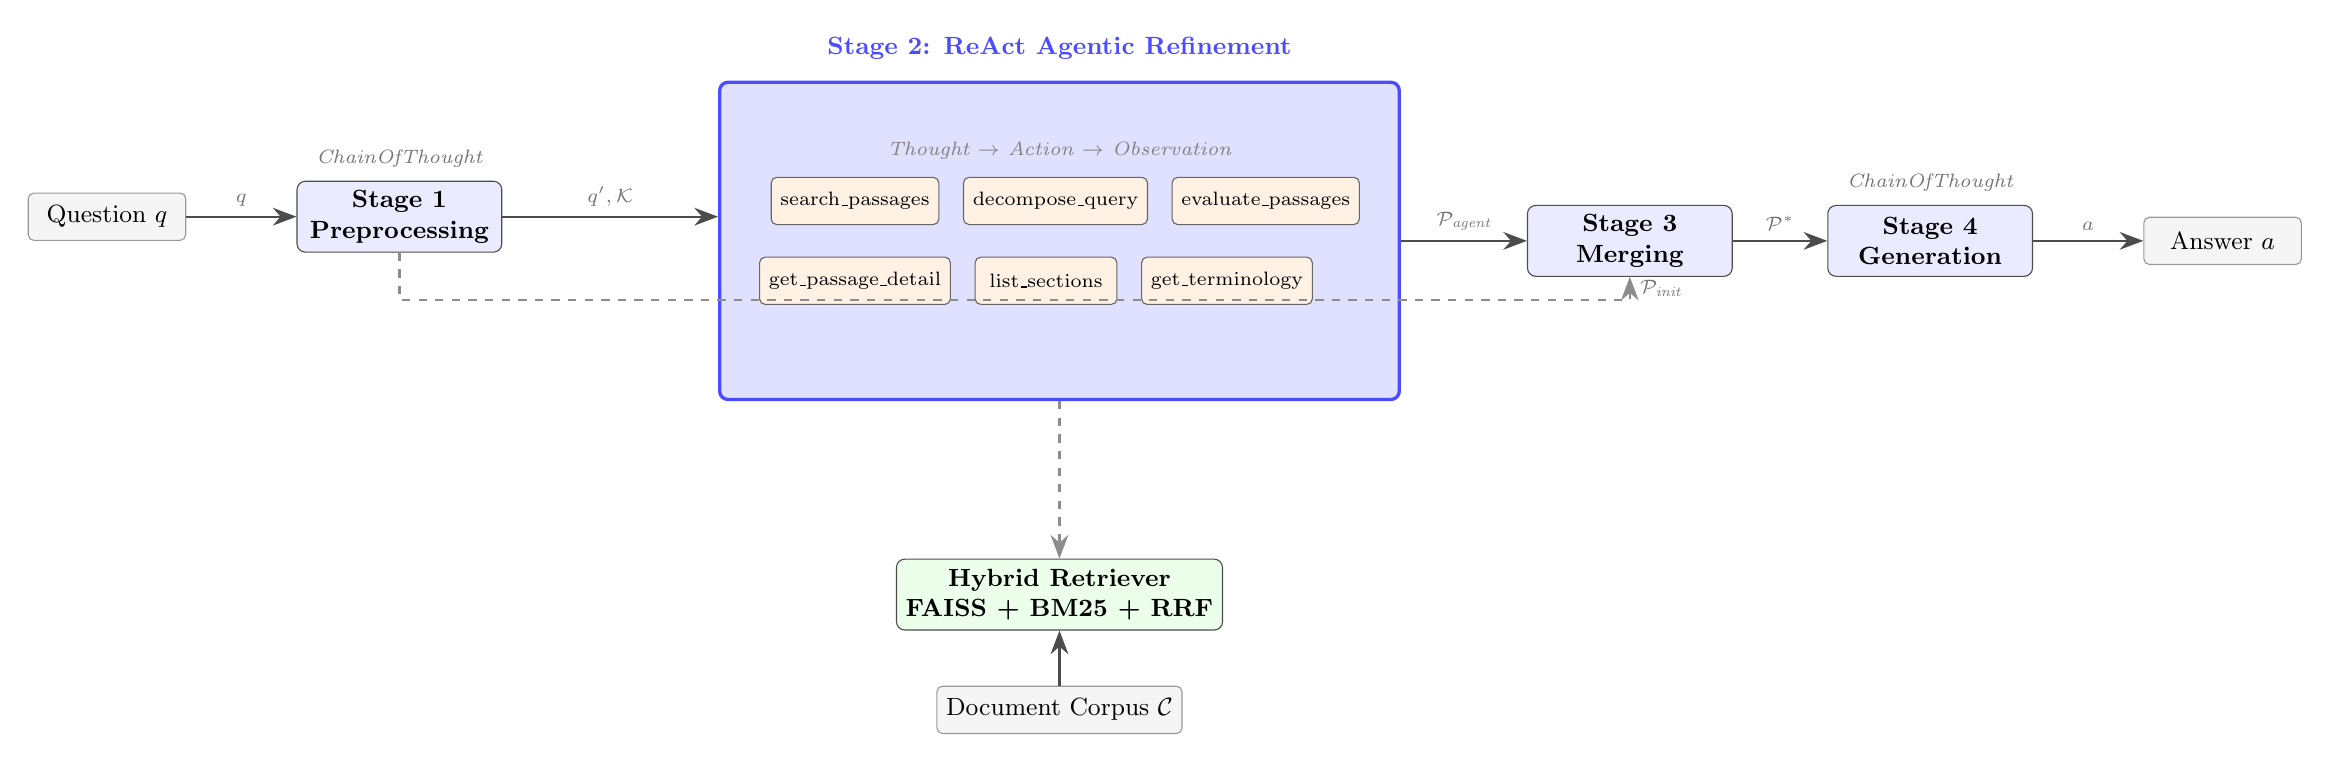
\begin{tikzpicture}[
    node distance=0.8cm and 1.2cm,
    >={Stealth[length=3mm]},
    stage/.style={rectangle, draw=black!70, fill=blue!8, rounded corners=3pt,
                  minimum width=2.6cm, minimum height=0.9cm, align=center,
                  font=\small\bfseries},
    tool/.style={rectangle, draw=black!60, fill=orange!10, rounded corners=2pt,
                 minimum width=1.8cm, minimum height=0.6cm, align=center,
                 font=\scriptsize},
    agent/.style={rectangle, draw=blue!70, fill=blue!12, rounded corners=3pt,
                  align=center, font=\small\bfseries, line width=1.2pt},
    io/.style={rectangle, draw=black!40, fill=gray!8, rounded corners=2pt,
               minimum width=2cm, minimum height=0.6cm, align=center,
               font=\small},
    arrow/.style={->, thick, black!70},
    dashedarrow/.style={->, dashed, thick, black!45},
    lbl/.style={font=\scriptsize\itshape, text=black!55},
]

% Row 1: Main pipeline flow
\node[io] (input) {Question $q$};
\node[stage, right=1.4cm of input] (preprocess) {Stage 1\\Preprocessing};
\node[lbl, above=0.05cm of preprocess] {ChainOfThought};

% Agent box — place tools first, then fit box around them
% Row 1 tools at a fixed position
\node[tool] (t1) at (9.5, 0.2) {search\_passages};
\node[tool, right=0.3cm of t1] (t2) {decompose\_query};
\node[tool, right=0.3cm of t2] (t3) {evaluate\_passages};
% Row 2 tools
\node[tool, below=0.4cm of t1] (t4) {get\_passage\_detail};
\node[tool, right=0.3cm of t4] (t5) {list\_sections};
\node[tool, right=0.3cm of t5] (t6) {get\_terminology};

% Agent box — fit around all tools with padding (extra top for subtitle)
\begin{scope}[on background layer]
\node[agent, fit=(t1)(t2)(t3)(t4)(t5)(t6),
      inner xsep=0.5cm, inner ysep=1.2cm] (agentbox) {};
\end{scope}
% Title above box, subtitle inside top area (above tools)
\node[font=\small\bfseries, text=blue!70, anchor=south] at ([yshift=0.15cm]agentbox.north) {Stage 2: ReAct Agentic Refinement};
\node[font=\scriptsize\itshape, text=black!50, anchor=south] at ([yshift=0.1cm]t1.north -| agentbox.center) {Thought $\to$ Action $\to$ Observation};

% Continue main flow
\node[stage, right=1.6cm of agentbox] (merge) {Stage 3\\Merging};
\node[stage, right=1.2cm of merge] (generate) {Stage 4\\Generation};
\node[lbl, above=0.05cm of generate] {ChainOfThought};
\node[io, right=1.4cm of generate] (output) {Answer $a$};

% Row 2: Retriever
\node[stage, below=2.0cm of agentbox, fill=green!8] (retriever) {Hybrid Retriever\\FAISS + BM25 + RRF};
\node[io, below=0.7cm of retriever] (corpus) {Document Corpus $\mathcal{C}$};

% === Arrows ===
% Main flow
\draw[arrow] (input) -- (preprocess) node[midway, above, lbl] {$q$};
\draw[arrow] (preprocess) -- (agentbox.west |- preprocess) node[midway, above, lbl] {$q', \mathcal{K}$};
\draw[arrow] (agentbox.east |- merge) -- (merge) node[midway, above, lbl] {$\mathcal{P}_{\text{agent}}$};
\draw[arrow] (merge) -- (generate) node[midway, above, lbl] {$\mathcal{P}^*$};
\draw[arrow] (generate) -- (output) node[midway, above, lbl] {$a$};

% Retriever connections
\draw[arrow] (corpus) -- (retriever);
\draw[dashedarrow] (agentbox.south) -- (retriever.north);

% Initial retrieval bypass to merge
\draw[dashedarrow] (preprocess.south) -- ++(0,-0.6) -| (merge.south)
    node[pos=0.75, right, lbl] {$\mathcal{P}_{\text{init}}$};

\end{tikzpicture}
}%
\caption{Overall architecture of \ours{}. The pipeline consists of four stages: (1)~query preprocessing, (2)~ReAct agentic refinement with six specialized tools, (3)~passage merging, and (4)~answer generation. Dashed arrows indicate the initial retrieval path and retriever connection.}
\label{fig:architecture}
\end{figure*}


% Figure 2: Pipeline Comparison — Naive vs CRAG vs Loop vs Agentic
\begin{figure*}[t]
\centering
\resizebox{0.95\textwidth}{!}{%
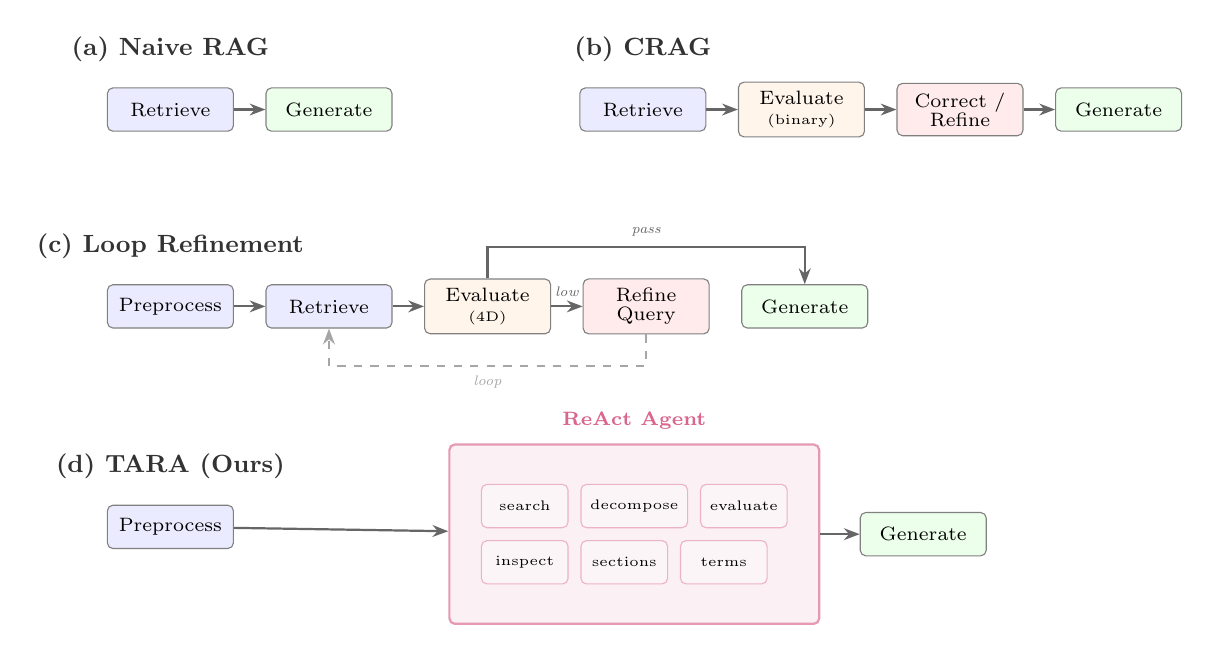
\begin{tikzpicture}[
    node distance=0.6cm and 0.5cm,
    >={Stealth[length=2mm]},
    box/.style={rectangle, draw=black!50, rounded corners=2pt,
                minimum width=1.6cm, minimum height=0.55cm, align=center,
                font=\scriptsize},
    pbox/.style={box, fill=blue!8},
    ebox/.style={box, fill=orange!8},
    gbox/.style={box, fill=green!8},
    abox/.style={box, fill=red!8},
    arrow/.style={->, thick, black!60},
    darrow/.style={->, dashed, thick, black!35},
    plabel/.style={font=\small\bfseries, text=black!80},
]

% === (a) Naive RAG ===
\node[plabel] (la) at (0, 0) {(a) Naive RAG};
\node[pbox, below=0.2cm of la] (a1) {Retrieve};
\node[gbox, right=0.4cm of a1] (a2) {Generate};
\draw[arrow] (a1) -- (a2);

% === (b) CRAG ===
\node[plabel] (lb) at (6, 0) {(b) CRAG};
\node[pbox, below=0.2cm of lb] (b1) {Retrieve};
\node[ebox, right=0.4cm of b1] (b2) {Evaluate\\[-1pt]{\tiny(binary)}};
\node[abox, right=0.4cm of b2] (b3) {Correct /\\[-1pt]Refine};
\node[gbox, right=0.4cm of b3] (b4) {Generate};
\draw[arrow] (b1) -- (b2);
\draw[arrow] (b2) -- (b3);
\draw[arrow] (b3) -- (b4);

% === (c) Loop Refinement ===
\node[plabel] (lc) at (0, -2.5) {(c) Loop Refinement};
\node[pbox, below=0.2cm of lc] (c1) {Preprocess};
\node[pbox, right=0.4cm of c1] (c2) {Retrieve};
\node[ebox, right=0.4cm of c2] (c3) {Evaluate\\[-1pt]{\tiny(4D)}};
\node[abox, right=0.4cm of c3] (c4) {Refine\\[-1pt]Query};
\node[gbox, right=0.4cm of c4] (c5) {Generate};
\draw[arrow] (c1) -- (c2);
\draw[arrow] (c2) -- (c3);
\draw[arrow] (c3) -- (c4) node[midway, above, font=\tiny\itshape] {low};
\draw[arrow] (c3.north) -- ++(0, 0.4) -| (c5.north) node[near start, above, font=\tiny\itshape] {pass};
\draw[darrow] (c4.south) -- ++(0, -0.4) -| (c2.south) node[near start, below, font=\tiny\itshape] {loop};

% === (d) AgenticRAG (Ours) ===
\node[plabel] (ld) at (0, -5.3) {(d) \ours{} (Ours)};
\node[pbox, below=0.2cm of ld] (d1) {Preprocess};

% Tools first, then fit box around them
\node[box, fill=purple!4, draw=purple!30, minimum width=1.1cm, font=\tiny]
    (dt1) at (4.5, -5.8) {search};
\node[box, fill=purple!4, draw=purple!30, minimum width=1.1cm, font=\tiny,
      right=0.15cm of dt1] (dt2) {decompose};
\node[box, fill=purple!4, draw=purple!30, minimum width=1.1cm, font=\tiny,
      right=0.15cm of dt2] (dt3) {evaluate};
\node[box, fill=purple!4, draw=purple!30, minimum width=1.1cm, font=\tiny,
      below=0.15cm of dt1] (dt4) {inspect};
\node[box, fill=purple!4, draw=purple!30, minimum width=1.1cm, font=\tiny,
      right=0.15cm of dt4] (dt5) {sections};
\node[box, fill=purple!4, draw=purple!30, minimum width=1.1cm, font=\tiny,
      right=0.15cm of dt5] (dt6) {terms};

% Agent box — fit around tools (background layer so tools stay visible)
\begin{scope}[on background layer]
\node[rectangle, draw=purple!40, fill=purple!6, rounded corners=2pt,
      line width=0.8pt, fit=(dt1)(dt2)(dt3)(dt4)(dt5)(dt6),
      inner xsep=0.4cm, inner ysep=0.5cm] (d2) {};
\end{scope}
\node[font=\scriptsize\bfseries, text=purple!60, anchor=south]
      at ([yshift=0.05cm]d2.north) {ReAct Agent};

\node[gbox, right=0.5cm of d2] (d3) {Generate};
\draw[arrow] (d1) -- (d2);
\draw[arrow] (d2) -- (d3);

\end{tikzpicture}
}%
\caption{Comparison of pipeline architectures. (a)~Naive RAG: single-pass retrieval. (b)~CRAG: binary evaluation with single-pass correction. (c)~Loop Refinement: fixed retrieve--evaluate--refine cycle. (d)~\ours{}: ReAct agent with six tools for adaptive refinement.}
\label{fig:pipeline_comparison}
\end{figure*}


Figure~\ref{fig:architecture} illustrates the \ours{} pipeline, and Figure~\ref{fig:pipeline_comparison} contrasts it with prior approaches. The pipeline consists of four stages:

\begin{enumerate}
    \item \textbf{Query Preprocessing.} The input question $q$ is rephrased into a standalone search query $q'$ and a set of search keywords $\mathcal{K}$ using a ChainOfThought module (DSPy \texttt{PreprocessSignature}). Optionally, a Hypothetical Document Embedding (HyDE)~\cite{gao2023hyde} query is generated for improved dense retrieval.

    \item \textbf{ReAct Agentic Refinement.} The preprocessed query is passed to a ReAct agent equipped with six tools (\S\ref{subsec:agent}). The agent iteratively searches, decomposes, evaluates, and inspects passages through autonomous reasoning. This stage replaces the fixed iterative loop in prior work.

    \item \textbf{Passage Merging.} Agent-selected passages are merged with initial retrieval results (from Stage 1) using priority-based deduplication: agent-refined passages take precedence, followed by initial results, capped at $M = 30$ passages.

    \item \textbf{Answer Generation.} A ChainOfThought generator (DSPy \texttt{QnAGenerate\-Signature}) produces the final answer conditioned on the merged passages, with adaptive response formatting based on question type.
\end{enumerate}

% ---------------------------------------------------------------------------
\subsection{ReAct Agent and Tool Design}
\label{subsec:agent}
% ---------------------------------------------------------------------------

The core of \ours{} is a ReAct agent~\cite{yao2023react} that interleaves reasoning (Thought) with tool execution (Action) and result observation (Observation).
Unlike fixed-loop refinement, the agent dynamically decides \emph{which} tools to call, \emph{how many} times, and \emph{when} to stop based on its assessment of the current retrieval state.

The agent operates through a DSPy Signature (the \texttt{AgenticRefinement\-Signature}) that specifies typed inputs and outputs.
The signature's docstring serves as a structured protocol, guiding the agent through a recommended sequence of steps while allowing deviations based on the agent's reasoning.

\subsubsection{Tool Set}
\label{subsubsec:tools}

The agent has access to six tools, each implemented as a closure over shared pipeline components (retriever, indexer, evaluator).
The first four are \emph{core tools} invoked on virtually every question; the remaining two are \emph{domain-adaptive auxiliary tools} whose utility depends on corpus characteristics (see RQ4 in \S\ref{subsec:rq4}):

\begin{enumerate}
    \item \textbf{\texttt{search\_passages}$(q, \mathcal{K})$}: Executes hybrid retrieval (FAISS + BM25 with RRF fusion) and returns passage previews (first 200 characters) to conserve context. This is the primary retrieval tool, called on average 3--4 times per question.

    \item \textbf{\texttt{decompose\_query}$(q)$}: Decomposes a complex multi-hop question into 2--4 independent sub-questions using a DSPy \texttt{DecomposeQuerySignature}. Returns a boolean \texttt{is\_multi\_hop} flag and the sub-question list.

    \item \textbf{\texttt{evaluate\_passages}$(q, \mathcal{P})$}: Assesses passage quality on four dimensions---Relevance (0--30), Coverage (0--25), Specificity (0--25), Sufficiency (0--20)---producing a total score $s \in [0, 100]$ with an action decision (\texttt{output}\slash\texttt{refine}) and refinement feedback. A mandatory fallback ensures this tool is called at least once per question.

    \item \textbf{\texttt{get\_passage\_detail}$(id)$}: Retrieves the full text of a passage by ID, enabling the agent to read complete content after identifying promising passages from search previews. This implements a progressive information disclosure strategy.

    \item \textbf{\texttt{list\_document\_sections}$(id)$}: Browses the hierarchical structure (sections, table of contents) of a source document, enabling structure-aware navigation for documents with rich organizational hierarchy.

    \item \textbf{\texttt{get\_terminology}$(term)$}: Maps user-facing terms to document-internal terminology, bridging vocabulary gaps between questions and corpus language.
\end{enumerate}

An optional \texttt{calculate} tool is available for domain-specific numerical computations (\eg, financial calculations) but is not part of the six core retrieval tools.

\subsubsection{Agent Protocol}
\label{subsubsec:protocol}

The agent's signature includes a structured protocol embedded in the docstring:

\begin{enumerate}
    \item Call \texttt{decompose\_query} to determine multi-hop structure.
    \item Call \texttt{search\_passages} with the initial query; if multi-hop, search each sub-question separately.
    \item Optionally call \texttt{get\_passage\_detail} on promising results.
    \item \textbf{Mandatory}: Call \texttt{evaluate\_passages} on the accumulated passage set.
    \item If score $< \tau$: use evaluation feedback to refine the query and search again.
    \item Call \texttt{finish} when quality is sufficient or further search is unlikely to improve results.
\end{enumerate}

The protocol is a recommendation, not a constraint---the agent may deviate based on its reasoning.
However, a mandatory evaluate fallback ensures that quality assessment is never entirely skipped: if the agent reaches \texttt{finish} without calling \texttt{evaluate\_passages}, the pipeline automatically runs the evaluation tool on the accumulated passages.

Figure~\ref{fig:react_example} shows an example agent trajectory for a 3-hop question.

% Figure 3: ReAct Agent Workflow Example
\begin{figure}[t]
\centering
\small
\begin{tikzpicture}[
    >={Stealth[length=2mm]},
    thought/.style={rectangle, draw=blue!50, fill=blue!5, rounded corners=2pt,
                    text width=5.8cm, align=left, font=\scriptsize,
                    inner sep=3pt},
    action/.style={rectangle, draw=orange!50, fill=orange!5, rounded corners=2pt,
                   text width=5.8cm, align=left, font=\scriptsize,
                   inner sep=3pt},
    obs/.style={rectangle, draw=green!50, fill=green!5, rounded corners=2pt,
                text width=5.8cm, align=left, font=\scriptsize,
                inner sep=3pt},
    stepnum/.style={circle, draw=black!40, fill=black!8, minimum size=0.4cm,
                 font=\scriptsize\bfseries},
    inbox/.style={below=0.03cm of},  % gap between boxes within a step
    stepgap/.style={below=0.35cm of}, % gap between steps
]

% Step 1 — T + A + O
\node[thought] (t1) at (3.3, 0) {\textbf{T:} Multi-hop question. Decompose first.};
\node[action, below=0.03cm of t1] (a1) {\textbf{A:} \texttt{decompose\_query}(``Who directed the film starring the actor born in Springfield?'')};
\node[obs, below=0.03cm of a1] (o1) {\textbf{O:} sub\_questions=[``actor born in Springfield?'', ``film starring actor?'', ``director?'']};
\node[stepnum] at (0, 0) {1};

% Step 2 — T + A + O
\node[thought, below=0.35cm of o1] (t2) {\textbf{T:} Search sub-questions for bridging facts.};
\node[action, below=0.03cm of t2] (a2) {\textbf{A:} \texttt{search\_passages}(``actor born in Springfield'')};
\node[obs, below=0.03cm of a2] (o2) {\textbf{O:} 5 passages. ``John Smith was born in Springfield, IL...''};
\node[stepnum] at (0 |- t2) {2};

% Step 3 — A + O
\node[action, below=0.35cm of o2] (a3) {\textbf{A:} \texttt{evaluate\_passages}(question, passages)};
\node[obs, below=0.03cm of a3] (o3) {\textbf{O:} Score 62/100, \textit{refine}. ``Missing director info.''};
\node[stepnum] at (0 |- a3) {3};

% Step 4 — A + O
\node[action, below=0.35cm of o3] (a4) {\textbf{A:} \texttt{search\_passages}(``film directed starring John Smith'')};
\node[obs, below=0.03cm of a4] (o4) {\textbf{O:} 3 passages. Score 85/100 $\to$ \texttt{finish}};
\node[stepnum] at (0 |- a4) {4};

\end{tikzpicture}
\caption{Example ReAct trajectory for a 3-hop question. T=Thought, A=Action, O=Observation. The agent decomposes, searches, evaluates, and refines based on feedback.}
\label{fig:react_example}
\end{figure}


% ---------------------------------------------------------------------------
\subsection{Self-Corrective Refinement Mechanism}
\label{subsec:refinement}
% ---------------------------------------------------------------------------

The self-corrective loop in \ours{} differs from prior work in three key aspects:

\paragraph{Adaptive Depth}
Rather than iterating a fixed number of times, the agent decides when to stop based on quality signals.
Simple questions may require only one search--evaluate cycle, while complex multi-hop questions trigger multiple decompose--search--evaluate iterations.
The maximum number of ReAct iterations is set to $I = 5$ to prevent unbounded execution.

\paragraph{Progressive Leniency}
The quality threshold decreases with each evaluation attempt to prevent over-iteration:
\begin{equation}
    \tau_{\text{eff}}^{(t)} = \tau - t \cdot \delta, \quad \delta = 5,
    \label{eq:progressive}
\end{equation}
where $\tau = 40$ is the base threshold.
This ensures the agent eventually terminates with the best available passages rather than continuing to search for marginally improved results.

\paragraph{Structured Feedback}
When the evaluation score falls below the threshold, the evaluation tool provides targeted feedback---suggested queries, keywords to add or remove---that directly informs the agent's next search action.
This feedback loop replaces generic retry logic with informed refinement.

% ---------------------------------------------------------------------------
\subsection{DSPy Declarative Pipeline}
\label{subsec:dspy}
% ---------------------------------------------------------------------------

The entire \ours{} pipeline is implemented using DSPy~\cite{khattab2024dspy}, a framework for programming LM-based systems through declarative \emph{Signatures} and composable \emph{Modules}.

\subsubsection{Signature Design}
\label{subsubsec:signatures}

Each pipeline stage is defined as a DSPy Signature with typed input and output fields:

{\small
\begin{itemize}
    \item \textbf{PreprocessSignature}: (question, history) $\rightarrow$ (rephrased\_question, keywords, topic)
    \item \textbf{EvaluationSignature}: (question, passages, retry\_count) $\rightarrow$ (scores$_{4D}$, action, feedback)
    \item \textbf{QnAGenerateSignature}: (question, passages) $\rightarrow$ (answer, footnotes)
    \item \textbf{DecomposeQuerySignature}: (question) $\rightarrow$ (is\_multi\_hop, sub\_questions)
    \item \textbf{AgenticRefinementSignature}: (question, query, keywords, $\tau$) $\rightarrow$ (passages, action)
\end{itemize}
}

The typed field descriptions serve as structured prompts, replacing hand-crafted JSON templates.
Each Signature's docstring provides task-specific instructions and scoring guidelines.

\subsubsection{Module Composition}
\label{subsubsec:modules}

Signatures are composed with DSPy modules:
\begin{itemize}
    \item \texttt{ChainOfThought}~\cite{wei2022chain}: Wraps the PreprocessSignature and QnAGenerateSignature to elicit step-by-step reasoning before outputs.
    \item \texttt{Predict}: Wraps the EvaluationSignature for direct structured output.
    \item \texttt{ReAct}: Wraps the AgenticRefinementSignature with tool integration, implementing the Thought--Action--Observation loop.
\end{itemize}

\subsubsection{Automatic Optimization}
\label{subsubsec:optimization}

DSPy enables automatic prompt optimization without modifying the pipeline code:

\begin{itemize}
    \item \textbf{BootstrapFewShot}~\cite{khattab2024dspy}: Collects successful execution traces as few-shot demonstrations. Each trace includes the full input--output chain, providing in-context examples that improve LM performance.

    \item \textbf{MIPROv2}~\cite{opsahl2024miprov2}: Generates and optimizes natural language instructions for each Signature using Bayesian surrogate models. It jointly optimizes instructions and few-shot examples across all pipeline modules.
\end{itemize}

Both optimizers use a training set of 50 examples with F1 score as the optimization metric.
The optimization cost is amortized: training is performed once, and the optimized prompts (few-shot demonstrations and/or instructions) are reused for all subsequent queries.

% ---------------------------------------------------------------------------
\subsection{Hybrid Retrieval}
\label{subsec:retrieval}
% ---------------------------------------------------------------------------

\ours{} uses a hybrid retrieval system combining dense and sparse search with Reciprocal Rank Fusion (RRF)~\cite{cormack2009rrf}:

\paragraph{Dense Retrieval}
Documents are embedded using a sentence transformer model and indexed with FAISS~\cite{johnson2019faiss} for approximate nearest neighbor search.
Given a query $q$, the dense retriever returns the top-$k$ passages by cosine similarity.

\paragraph{Sparse Retrieval}
BM25~\cite{robertson2009bm25} provides lexical matching for keyword-heavy queries, particularly effective for entity names and technical terms that may not be well-captured by dense embeddings.

\paragraph{Reciprocal Rank Fusion}
The results from both retrievers are combined using RRF:
\begin{equation}
    \text{RRF}(d) = \sum_{r \in \{dense, sparse\}} \frac{1}{\kappa + \text{rank}_r(d)},
    \label{eq:rrf}
\end{equation}
where $\kappa = 60$ is a smoothing constant and $\text{rank}_r(d)$ is the rank of document $d$ in retriever $r$'s result list.
The fused ranking is used as the final retrieval output, with the top $k = 50$ results returned per query.


%% ====================================================================
\section{Experimental Setup}
\label{sec:setup}
%% ====================================================================

% ===========================================================================
% Section 4: Experimental Setup
% ===========================================================================

% ---------------------------------------------------------------------------
\subsection{Datasets}
\label{subsec:datasets}
% ---------------------------------------------------------------------------

We evaluate \ours{} on four datasets spanning multi-hop reasoning and enterprise document QA, summarized in Table~\ref{tab:datasets}.
For a comprehensive survey of multi-hop QA methods, we refer readers to Mavi et al.~\cite{mavi2024multihop}.

\begin{table}[t]
\centering
\caption{Dataset statistics. Multi-hop QA datasets include context paragraphs as self-contained retrieval corpora. FinanceBench provides evidence passages from SEC filings.}
\label{tab:datasets}
\begin{tabular}{lcccc}
\toprule
\textbf{Dataset} & \textbf{Domain} & \textbf{Hops} & \textbf{Answer Type} & \textbf{Source} \\
\midrule
HotpotQA & Wikipedia & 2 & Extractive & \cite{yang2018hotpotqa} \\
2WikiMultiHopQA & Wikipedia & 2--4 & Extractive & \cite{ho2020wiki2multi} \\
MuSiQue & Wikipedia & 2--4 & Extractive & \cite{trivedi2022musique} \\
FinanceBench & SEC filings & 1--3 & Analytical & \cite{financebench2023} \\
\bottomrule
\end{tabular}
\end{table}

\textbf{HotpotQA}~\cite{yang2018hotpotqa} is a 2-hop multi-hop QA dataset over Wikipedia, where each question requires reasoning over two supporting paragraphs mixed with distractor paragraphs.
We use the \texttt{distractor} setting from the validation split.

\textbf{2WikiMultiHopQA}~\cite{ho2020wiki2multi} extends multi-hop reasoning to 2--4 hops, with questions constructed through systematic composition of single-hop questions from two Wikipedia articles.
This dataset tests deeper reasoning chains than HotpotQA.

\textbf{MuSiQue}~\cite{trivedi2022musique} (\textbf{Mu}lti-hop \textbf{Si}ngle-hop \textbf{Que}stion composition) provides 2--4 hop questions with controlled compositionality, designed to resist shortcut reasoning.
It is generally considered the most challenging of the three multi-hop datasets.

\textbf{FinanceBench}~\cite{financebench2023} provides questions over real SEC filings (10-K, 10-Q, 8-K reports), requiring numerical reasoning and domain-specific terminology understanding.
Related financial QA benchmarks include FinQA~\cite{chen2021finqa} for numerical reasoning over financial tables and DocFinQA~\cite{reddy2024docfinqa} for long-context financial documents.
This dataset evaluates practical applicability in enterprise settings where external web search is unavailable.

Each dataset provides its own context paragraphs (supporting documents plus distractors), which we use as the retrieval corpus.
We build separate FAISS and BM25 indices per dataset.

% ---------------------------------------------------------------------------
\subsection{Baselines}
\label{subsec:baselines}
% ---------------------------------------------------------------------------

We compare \ours{} against four baselines of increasing complexity, all sharing the same retrieval infrastructure and generation model for fair comparison:

\begin{enumerate}
    \item \textbf{Naive RAG}: Single-pass retrieve-and-generate with no evaluation or correction. Uses the same hybrid retriever and ChainOfThought generator.

    \item \textbf{CRAG Replica}~\cite{yan2024crag}: Reproduces the core CRAG mechanism with binary relevance evaluation (correct/incorrect/ambiguous), knowledge refinement via strip decomposition, and internal search fallback.
    Two adaptations are necessary for fair comparison: (a)~CRAG's web search fallback is replaced with internal corpus re-retrieval, as our evaluation setting assumes a closed corpus without external web access---a realistic constraint for enterprise deployments; (b)~the original fine-tuned T5-large evaluator is replaced with LLM-based evaluation using the same model as other pipelines, ensuring the same compute class across all baselines.
    These adaptations disadvantage CRAG relative to its original design; we discuss this in \S\ref{subsec:rq1}.

    \item \textbf{Single-Pass}: Preprocessing (query rephrasing + keyword extraction) followed by hybrid retrieval and generation. Includes one evaluation step but no iterative refinement.

    \item \textbf{Loop Refinement}: Fixed for-loop self-corrective pipeline implementing iterative retrieval, 4D quality evaluation, and targeted query refinement. Iterates up to $T = 3$ times based on evaluation scores. This represents the non-agentic version of our refinement approach.
\end{enumerate}

The key difference between Loop Refinement and \ours{} is the refinement strategy: Loop follows a predetermined retrieve--evaluate--refine sequence, while \ours{} autonomously selects tools and decides when to stop through ReAct reasoning.

% ---------------------------------------------------------------------------
\subsection{Evaluation Metrics}
\label{subsec:metrics}
% ---------------------------------------------------------------------------

We use three primary metrics and one secondary metric:

\paragraph{Primary Metrics}

\begin{itemize}
    \item \textbf{Exact Match (EM)}: Binary indicator of whether the normalized prediction exactly matches the reference answer, after lowercasing, removing articles/punctuation/whitespace, and stripping footnote markers.

    \item \textbf{Token-level F1}: Harmonic mean of token-level precision and recall between the normalized prediction and reference, following the standard SQuAD evaluation protocol. This captures partial credit for partially correct answers.

    \item \textbf{LLM-as-Judge}~\cite{zheng2023judging}: A DSPy-based correctness judge that evaluates whether the prediction is semantically equivalent to the reference answer, using the same evaluation model. This captures cases where the answer is correct but lexically different from the reference (\eg, ``Dutch'' vs.\ ``the Netherlands'').
\end{itemize}

\paragraph{Secondary Metric}

\begin{itemize}
    \item \textbf{ROUGE-L}~\cite{lin2004rouge}: Longest common subsequence-based overlap score, providing an alternative view of answer quality. Reported in supplementary material.
\end{itemize}

We also report \textbf{average latency} per question to quantify the computational cost--quality trade-off.
We note that alternative evaluation frameworks exist for RAG systems, including RAGAS~\cite{es2024ragas} for component-level evaluation, FActScore~\cite{min2023factscore} for fine-grained factual precision, and BERTScore~\cite{zhang2020bertscore} for semantic similarity.
We focus on EM, F1, and LLM-as-Judge as they directly measure answer correctness and are standard in the multi-hop QA literature.

% ---------------------------------------------------------------------------
\subsection{Implementation Details}
\label{subsec:implementation}
% ---------------------------------------------------------------------------

\paragraph{Models}
Primary experiments use Gemini Flash Lite~\cite{geminiteam2023gemini}\footnote{Model~ID: \texttt{gemini/gemini-3.1-flash-lite-preview}} for all four LLM slots (preprocessing, evaluation, generation, agent) via LiteLLM.
For cross-model validation (RQ1), we replicate experiments with gpt-5-mini\footnote{Model~ID: \texttt{gpt-5-mini}, \texttt{reasoning\_effort=low}.}, a reasoning-oriented model from a different architecture family, to assess generalizability.
An independent LLM-as-Judge (gpt-4.1-nano) evaluates answer correctness by comparing predicted and reference answers via a DSPy-based correctness signature.
The judge receives the question, reference answer, and predicted answer, and outputs a binary correctness decision with chain-of-thought reasoning.
This model is independent of all pipeline models to avoid evaluation bias; it captures semantic equivalences that token-level F1 misses (\eg, ``Dutch'' vs.\ ``the Netherlands'').
Embeddings use all-MiniLM-L6-v2 (384 dimensions) via sentence-trans\-formers~\cite{reimers2019sentence}.
Temperature is set to 0.0 for reproducibility.

\paragraph{Retrieval}
FAISS indices use inner product search with L2-normalized embeddings (equivalent to cosine similarity).
BM25 uses the rank-bm25 library with default parameters.
RRF fusion uses $k = 60$.
The retriever returns top-$k = 50$ results per query, with a maximum of $M = 30$ accumulated passages.

\paragraph{Agent}
The ReAct agent operates with a maximum of $I = 5$ reasoning--action iterations.
The quality threshold is $\tau = 40$ with progressive leniency decrement $\delta = 5$ per evaluation attempt (minimum effective threshold: 20).
The maximum retry count for the evaluation tool is $T = 3$.
The maximum accumulated passages is $M = 30$.

\paragraph{DSPy Optimization}
BootstrapFewShot and MIPROv2 optimizers use a training set of 50 examples per dataset, with 20 reserved for validation and the remainder for testing ($N = 130$ for multi-hop datasets, $N = 80$ for FinanceBench).
Token-level F1 serves as the optimization metric.
Optimized prompts include up to 4 few-shot demonstrations.

\paragraph{Infrastructure}
Experiments run on a single machine with Python 3.11, DSPy 3.1+, and FAISS-CPU.
All code, configurations, and experiment scripts are available at \url{[anonymized]}.

\paragraph{Sample size and statistical testing}
Main experiments use $n = 200$ samples per dataset, with FinanceBench evaluated on the full dataset ($n = 150$).
Statistical significance is assessed via paired bootstrap testing~\cite{efron1993bootstrap} with 10,000 resamples and Bonferroni correction for multiple comparisons.
We report 95\% bootstrap confidence intervals for all primary comparisons.

\paragraph{Reproducibility}
All experiments use a fixed random seed (42) for dataset sampling.
Configuration is managed through YAML files with per-experiment overrides.
The entire pipeline---from dataset preparation through index building to experiment execution---is automated via CLI scripts.


%% ====================================================================
\section{Results and Analysis}
\label{sec:results}
%% ====================================================================

% ===========================================================================
% Section 5: Results and Analysis
% ===========================================================================

This section presents the main experimental results.
All experiments use $n = 200$ samples per dataset (FinanceBench: $n = 150$, full dataset) unless otherwise noted.
We address three research questions: RQ1 compares \ours{} against baselines (\S\ref{subsec:rq1}), RQ2 analyzes the agent's tool usage patterns (\S\ref{subsec:rq2}), and RQ5 evaluates DSPy optimization effects (\S\ref{subsec:rq5}).
Ablation studies for RQ3 (evaluation tool variants) and RQ4 (structure-aware tools) are presented in \S\ref{sec:ablation}.

% ---------------------------------------------------------------------------
\subsection{RQ1: Agentic vs.\ Baseline Pipelines}
\label{subsec:rq1}
% ---------------------------------------------------------------------------

\textbf{Does ReAct-based agentic refinement improve answer quality compared to fixed-loop refinement and single-pass baselines?}

Table~\ref{tab:rq1_main} and Figure~\ref{fig:rq1_f1} present the main results across four datasets using Gemini Flash Lite.

% Figure: RQ1 F1 Comparison (Gemini Flash Lite, n=200)
\begin{figure*}[t]
\centering
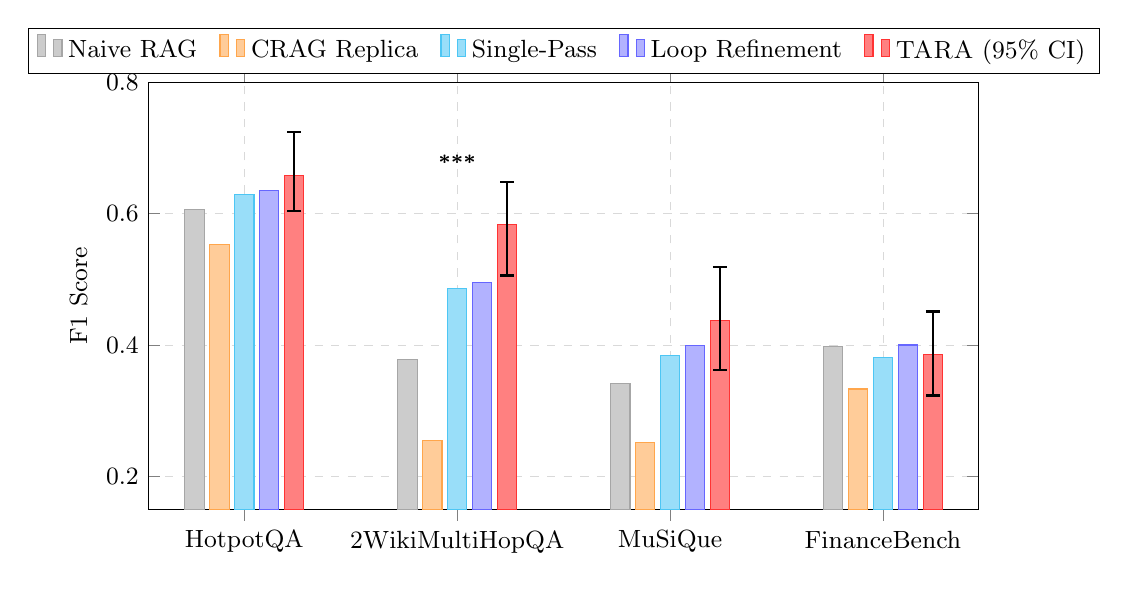
\begin{tikzpicture}
\begin{axis}[
    ybar,
    bar width=7pt,
    width=\textwidth,
    height=7cm,
    ylabel={F1 Score},
    symbolic x coords={HotpotQA, 2WikiMultiHopQA, MuSiQue, FinanceBench},
    xtick=data,
    ymin=0.15, ymax=0.80,
    legend style={
        at={(0.5,1.02)},
        anchor=south,
        legend columns=5,
        font=\small,
        /tikz/every even column/.append style={column sep=6pt}
    },
    ylabel style={font=\small},
    xticklabel style={font=\small},
    yticklabel style={font=\small},
    enlarge x limits=0.15,
    grid=major,
    grid style={dashed, gray!30},
    major grid style={line width=0.3pt},
]

% Naive RAG
\addplot[fill=gray!40, draw=gray!70] coordinates {
    (HotpotQA, 0.606)
    (2WikiMultiHopQA, 0.378)
    (MuSiQue, 0.342)
    (FinanceBench, 0.398)
};

% CRAG Replica
\addplot[fill=orange!40, draw=orange!70] coordinates {
    (HotpotQA, 0.553)
    (2WikiMultiHopQA, 0.255)
    (MuSiQue, 0.251)
    (FinanceBench, 0.333)
};

% Single-Pass
\addplot[fill=cyan!40, draw=cyan!70] coordinates {
    (HotpotQA, 0.630)
    (2WikiMultiHopQA, 0.486)
    (MuSiQue, 0.384)
    (FinanceBench, 0.381)
};

% Loop Refinement
\addplot[fill=blue!30, draw=blue!60] coordinates {
    (HotpotQA, 0.636)
    (2WikiMultiHopQA, 0.495)
    (MuSiQue, 0.399)
    (FinanceBench, 0.400)
};

% TARA (Agentic) with 95% bootstrap CI
% CI: Hot [.604,.725], 2Wiki [.506,.648], Mus [.362,.519], Fin [.323,.451]
% error minus = mean - lower, error plus = upper - mean
\addplot[
    fill=red!50, draw=red!80,
    error bars/.cd,
    y dir=both,
    y explicit,
    error bar style={black, thick},
    error mark options={rotate=90, mark size=2.5pt, thick},
] table [
    x=x, y=y,
    y error plus=ep,
    y error minus=em,
    col sep=comma,
] {
x,              y,     ep,    em
HotpotQA,       0.658, 0.067, 0.054
2WikiMultiHopQA,0.584, 0.064, 0.078
MuSiQue,        0.438, 0.081, 0.076
FinanceBench,   0.386, 0.065, 0.063
};

\legend{Naive RAG, CRAG Replica, Single-Pass, Loop Refinement, \ours{} (95\% CI)}

% Significance annotation
\node[font=\scriptsize\bfseries, anchor=south, yshift=1pt]
    at (axis cs:2WikiMultiHopQA, 0.648) {***};

\end{axis}
\end{tikzpicture}
\caption{F1 comparison across four datasets (Gemini Flash Lite, $n = 200$). \ours{} achieves the highest F1 on three of four datasets, with statistically significant improvement on 2WikiMultiHopQA ($p < 0.001$). Error bars on \ours{} indicate 95\% bootstrap confidence intervals (10,000 resamples; Table~\ref{tab:rq1_significance}). On FinanceBench, all iterative methods perform comparably (retrieval space saturation).}
\label{fig:rq1_f1}
\end{figure*}


\begin{table*}[t]
\centering
\caption{Main results (RQ1, Gemini Flash Lite). Best result per dataset in \textbf{bold}. $n = 200$ per dataset (FinanceBench: $n = 150$, full dataset). LLM-as-Judge uses gpt-4.1-nano as an independent evaluator.}
\label{tab:rq1_main}
\resizebox{\textwidth}{!}{%
\begin{tabular}{l ccc ccc ccc ccc}
\toprule
& \multicolumn{3}{c}{\textbf{HotpotQA}} & \multicolumn{3}{c}{\textbf{2WikiMultiHopQA}} & \multicolumn{3}{c}{\textbf{MuSiQue}} & \multicolumn{3}{c}{\textbf{FinanceBench}} \\
\cmidrule(lr){2-4} \cmidrule(lr){5-7} \cmidrule(lr){8-10} \cmidrule(lr){11-13}
\textbf{Pipeline} & EM & F1 & Judge & EM & F1 & Judge & EM & F1 & Judge & EM & F1 & Judge \\
\midrule
Naive RAG        & .445 & .606 & .700 & .275 & .378 & .400 & .235 & .342 & .335 & .167 & .398 & \textbf{.580} \\
CRAG Replica     & .400 & .553 & .645 & .130 & .255 & .320 & .175 & .251 & .225 & .107 & .333 & .487 \\
Single-Pass      & .470 & .630 & .720 & .375 & .486 & .495 & .280 & .384 & .360 & .160 & .381 & .507 \\
Loop Refinement  & .480 & .636 & .730 & .380 & .495 & .505 & .300 & .399 & .380 & \textbf{.180} & \textbf{.400} & .533 \\
\textbf{\ours{}} & \textbf{.505} & \textbf{.658} & \textbf{.765} & \textbf{.470} & \textbf{.584} & \textbf{.645} & \textbf{.330} & \textbf{.438} & \textbf{.405} & .153 & .386 & .527 \\
\midrule
\multicolumn{1}{r}{\textit{$\Delta$ vs.\ Loop}} & $+.025$ & $+.022$ & $+.035$ & $+.090$ & $+.089$ & $+.140$ & $+.030$ & $+.039$ & $+.025$ & $-.027$ & $-.014$ & $-.006$ \\
\bottomrule
\end{tabular}
}% end resizebox
\end{table*}

\paragraph{Complex multi-hop questions}
\ours{} achieves the best performance on both complex multi-hop datasets: 2WikiMultiHopQA (F1 0.584, $+0.089$ over Loop Refinement) and MuSiQue (F1 0.438, $+0.039$ over Loop).
These improvements are consistent across all three metrics (EM, F1, Judge), indicating genuine quality gains rather than metric-specific artifacts.
The LLM-as-Judge scores show the largest gaps on 2WikiMultiHopQA ($+0.140$), where the judge identifies correct multi-hop reasoning even when token overlap is moderate.
As we show in \S\ref{subsubsec:significance}, the 2WikiMultiHopQA improvement is statistically significant ($p < 0.001$) across all baseline comparisons.

\paragraph{Simple 2-hop questions}
On HotpotQA, \ours{} leads across all metrics (F1 0.658, EM 0.505, Judge 0.765), but the margin over Loop Refinement is small (F1 $+0.022$).
This suggests that 2-hop questions---where the required evidence can typically be retrieved in one or two search passes---do not fully exercise the agent's adaptive refinement capabilities.
The overhead of multi-step ReAct reasoning provides limited benefit when a single well-preprocessed retrieval pass is already sufficient.

\paragraph{Enterprise documents}
On FinanceBench, Loop Refinement marginally outperforms \ours{} in F1 (0.400 vs.\ 0.386, $\Delta = -0.014$) and EM (0.180 vs.\ 0.153).
Notably, Naive RAG achieves the highest Judge score (0.580), outperforming all iterative methods.
This pattern---where iterative refinement does \emph{not} improve and may slightly degrade answer quality---suggests a boundary condition for our approach.
We analyze this effect in detail in \S\ref{subsec:boundary}, attributing it to retrieval space saturation in FinanceBench's small corpus (211 passages).

\paragraph{CRAG Replica underperformance}
The CRAG Replica consistently ranks lowest, which is expected: our implementation replaces CRAG's web search fallback with internal re-retrieval (to match our enterprise-constrained setting) and uses LLM-based evaluation instead of a fine-tuned T5-large evaluator.
These architectural constraints substantially disadvantage the CRAG approach.

\paragraph{Key finding}
The agentic advantage is \emph{complexity-dependent}: improvements grow with question complexity (number of reasoning hops and retrieval difficulty), while simple questions and small-corpus settings show no benefit.
This pattern is consistent with the hypothesis that autonomous tool selection provides value primarily when the retrieval task requires adaptive strategy.

% ---------------------------------------------------------------------------
\subsubsection{Statistical Significance}
\label{subsubsec:significance}
% ---------------------------------------------------------------------------

To rigorously assess the reliability of observed differences, we perform paired bootstrap significance testing~\cite{efron1993bootstrap} with 10,000 resamples and Bonferroni correction for multiple comparisons.
Table~\ref{tab:rq1_significance} reports 95\% confidence intervals for \ours{} and pairwise comparisons against each baseline.

\begin{table*}[t]
\centering
\caption{Statistical significance (F1, paired bootstrap test, 10,000 resamples, Bonferroni-corrected $\alpha = 0.0125$). Top row: \ours{} F1 with 95\% bootstrap confidence interval. Lower rows: F1 difference $\Delta$ vs.\ each baseline (from Table~\ref{tab:rq1_main}); $p$-values from paired bootstrap. Significance: $^{***}p < 0.001$.}
\label{tab:rq1_significance}
\resizebox{\textwidth}{!}{%
\begin{tabular}{l cccc}
\toprule
& \textbf{HotpotQA} & \textbf{2WikiMultiHopQA} & \textbf{MuSiQue} & \textbf{FinanceBench} \\
\midrule
\ours{} F1 [95\% CI] & .658\;[.604,\;.725] & .584\;[.506,\;.648] & .438\;[.362,\;.519] & .386\;[.323,\;.451] \\
\midrule
$\Delta$ vs.\ Loop       & $+.022$           & $+.089^{***}$      & $+.039$           & $-.014$           \\
$\Delta$ vs.\ CRAG       & $+.105^{***}$     & $+.329^{***}$      & $+.187^{***}$     & $+.053$           \\
$\Delta$ vs.\ Single     & $+.028$           & $+.098^{***}$      & $+.054$           & $+.005$           \\
$\Delta$ vs.\ Naive      & $+.052$           & $+.206^{***}$      & $+.096^{***}$     & $-.012$           \\
\bottomrule
\end{tabular}
}% end resizebox
\end{table*}

\paragraph{2WikiMultiHopQA: strongest evidence}
\ours{} achieves statistically significant improvement over \emph{all four baselines} on 2WikiMultiHopQA ($p < 0.001$ in each case), with the largest effect against CRAG ($\Delta = +0.329$).
The 95\% confidence interval [$0.506, 0.648$] does not overlap with the confidence intervals of Loop [$0.433, 0.557$] or CRAG [$0.209, 0.305$], providing strong evidence that the improvement is not due to sampling variability.

\paragraph{MuSiQue: significant vs.\ weaker baselines}
Against CRAG ($+0.187$, $p < 0.001$) and Naive ($+0.096$, $p < 0.001$), the improvement is significant.
Against Loop ($+0.039$) and Single-Pass ($+0.054$), the positive trend does not reach significance, indicating that the refinement mechanisms converge for 3--4 hop questions that overlap in difficulty.

\paragraph{HotpotQA: comparable performance}
No pairwise comparison reaches significance except against CRAG ($+0.105$, $p < 0.001$), confirming that 2-hop questions do not discriminate between refinement approaches.

\paragraph{FinanceBench: no significant differences}
All pairwise comparisons are non-significant, with confidence intervals substantially overlapping.
The marginally negative delta against Loop ($-0.014$) is well within noise.
This statistical confirmation of the null result is consistent with the retrieval space saturation hypothesis discussed in \S\ref{subsec:boundary}.

% ---------------------------------------------------------------------------
\subsubsection{Cross-Model Validation}
\label{subsubsec:crossmodel}
% ---------------------------------------------------------------------------

To assess whether the observed patterns are model-dependent, we replicate the RQ1 experiment using gpt-5-mini\footnote{Model~ID: \texttt{gpt-5-mini}, with \texttt{reasoning\_effort=low}.}, a reasoning-oriented model from a different provider and architecture family.
Table~\ref{tab:rq1_crossmodel} presents the results.

\begin{table*}[t]
\centering
\caption{Cross-model validation (RQ1, gpt-5-mini). $n = 200$ per dataset (FinanceBench: $n = 150$). LLM-as-Judge: gpt-4.1-nano (same independent judge as Gemini experiments). Best per dataset in \textbf{bold}.}
\label{tab:rq1_crossmodel}
\resizebox{\textwidth}{!}{%
\begin{tabular}{l ccc ccc ccc ccc}
\toprule
& \multicolumn{3}{c}{\textbf{HotpotQA}} & \multicolumn{3}{c}{\textbf{2WikiMultiHopQA}} & \multicolumn{3}{c}{\textbf{MuSiQue}} & \multicolumn{3}{c}{\textbf{FinanceBench}} \\
\cmidrule(lr){2-4} \cmidrule(lr){5-7} \cmidrule(lr){8-10} \cmidrule(lr){11-13}
\textbf{Pipeline} & EM & F1 & Judge & EM & F1 & Judge & EM & F1 & Judge & EM & F1 & Judge \\
\midrule
Naive RAG        & .485 & .657 & .755 & .335 & .400 & .405 & .310 & .441 & .425 & .140 & .321 & \textbf{.540} \\
CRAG Replica     & \textbf{.535} & \textbf{.698} & .780 & \textbf{.550} & \textbf{.637} & \textbf{.655} & .370 & .491 & .460 & \textbf{.147} & \textbf{.343} & .520 \\
Single-Pass      & .505 & .678 & .735 & .390 & .465 & .485 & \textbf{.375} & .504 & .490 & .140 & .308 & .480 \\
Loop Refinement  & .510 & .689 & .750 & .425 & .510 & .540 & .370 & .505 & .485 & .160 & .328 & .507 \\
\textbf{\ours{}} & .510 & .697 & \textbf{.790} & .485 & .551 & .560 & \textbf{.375} & \textbf{.516} & \textbf{.505} & .133 & .317 & .513 \\
\midrule
\multicolumn{1}{r}{\textit{$\Delta$ vs.\ CRAG}} & $-.025$ & $-.001$ & $+.010$ & $-.065$ & $-.086$ & $-.095$ & $+.005$ & $+.025$ & $+.045$ & $-.014$ & $-.026$ & $-.007$ \\
\bottomrule
\end{tabular}
}% end resizebox
\end{table*}

\paragraph{Model--pipeline interaction effect}
The cross-model experiment reveals a striking reversal: with gpt-5-mini, CRAG Replica outperforms \ours{} on 2WikiMultiHopQA (F1 0.637 vs.\ 0.551, $p = 0.004$) and FinanceBench (F1 0.343 vs.\ 0.317, $p = 0.042$).
This contrasts sharply with the Gemini results, where \ours{} leads on both datasets.
The reversal is driven by what we term \emph{Reasoning Model Refusal Asymmetry}: the reasoning capabilities of gpt-5-mini lead it to apply higher evidentiary standards within the ReAct framework, resulting in a 30\% answer refusal rate on 2WikiMultiHopQA (compared to 18\% for CRAG).
CRAG's rigid judge--correct--generate pipeline precludes refusal, ensuring an answer is always produced.
We analyze this phenomenon in detail in \S\ref{subsec:model_interaction}.

\paragraph{Consistent findings}
Despite the model--pipeline interaction, several patterns remain consistent across both models:
(1)~\ours{} leads on MuSiQue (F1 0.516, Judge 0.505), the hardest multi-hop dataset;
(2)~Naive RAG achieves the highest Judge score on FinanceBench with both models (0.580 for Gemini, 0.540 for gpt-5-mini);
(3)~HotpotQA shows compressed performance ranges with both models.
The LLM-as-Judge also resolves an apparent tie on HotpotQA: \ours{} achieves 0.790 vs.\ CRAG's 0.780, suggesting subtle quality advantages that F1 cannot capture.

% ---------------------------------------------------------------------------
\subsubsection{Latency Analysis}
\label{subsubsec:latency}
% ---------------------------------------------------------------------------

Table~\ref{tab:latency} reports average per-question latency for the Gemini configuration.

\begin{table}[t]
\centering
\caption{Average latency per question (seconds, Gemini Flash Lite, $\tau = 40$). Latency is dominated by LLM API calls; the agent averages 5--6 tool invocations per question.}
\label{tab:latency}
\begin{tabular}{lcccc}
\toprule
\textbf{Pipeline} & \textbf{HotpotQA} & \textbf{2Wiki} & \textbf{MuSiQue} & \textbf{Finance} \\
\midrule
Naive RAG       & 0.5 & 0.3 & 0.3 & 0.3 \\
CRAG Replica    & 0.4 & 0.1 & 0.1 & 0.1 \\
Single-Pass     & 4.2 & 3.0 & 3.5 & 4.9 \\
Loop Refinement & 3.1 & 1.7 & 3.6 & 2.7 \\
\textbf{\ours{}} & 14.9 & 13.6 & 15.2 & 16.8 \\
\bottomrule
\end{tabular}
\end{table}

\ours{} requires 14--17 seconds per question, approximately 4--5$\times$ slower than Loop Refinement and 30--50$\times$ slower than Naive RAG.
This overhead stems from the ReAct reasoning loop: each iteration involves LLM inference for thought generation, tool selection, and observation processing.
With an average of 5.4--6.2 tool calls per question (see \S\ref{subsec:rq2}), the agent performs substantially more LLM calls than the fixed-loop approach.
With gpt-5-mini, latency increases further to 45.7s per question on 2WikiMultiHopQA due to the model's reasoning overhead. CRAG requires 147.8s per question with gpt-5-mini, as its multi-stage pipeline involves 45.2 LLM calls per question.
We discuss the latency--quality trade-off and practical implications in \S\ref{sec:discussion}.

% ---------------------------------------------------------------------------
\subsection{RQ2: Tool Usage and Trajectory Analysis}
\label{subsec:rq2}
% ---------------------------------------------------------------------------

\textbf{How does the ReAct agent use its tools, and what behavioral patterns emerge?}

% ---------------------------------------------------------------------------
\subsubsection{Tool Frequency}
\label{subsubsec:tool_freq}
% ---------------------------------------------------------------------------

Table~\ref{tab:tool_usage} and Figure~\ref{fig:tool_usage} report the average number of tool calls per question across all four datasets.

% Figure: Tool Usage Heatmap (RQ2)
\begin{figure}[t]
\centering
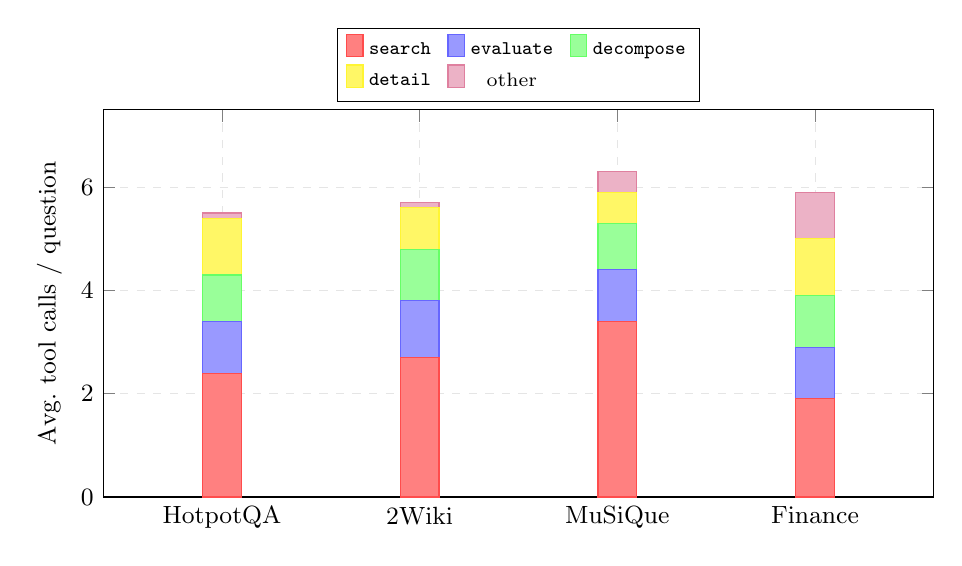
\begin{tikzpicture}
\begin{axis}[
    ybar stacked,
    bar width=14pt,
    width=\columnwidth,
    height=6.5cm,
    ylabel={Avg.\ tool calls / question},
    symbolic x coords={HotpotQA, 2Wiki, MuSiQue, Finance},
    xtick=data,
    xticklabel style={font=\small},
    ylabel style={font=\small},
    yticklabel style={font=\small},
    ymin=0, ymax=7.5,
    legend style={
        at={(0.5,1.02)},
        anchor=south,
        legend columns=3,
        font=\scriptsize,
        /tikz/every even column/.append style={column sep=4pt}
    },
    enlarge x limits=0.2,
    grid=major,
    grid style={dashed, gray!20},
    major grid style={line width=0.2pt},
]

% search_passages
\addplot[fill=red!50, draw=red!70] coordinates {
    (HotpotQA, 2.4)
    (2Wiki, 2.7)
    (MuSiQue, 3.4)
    (Finance, 1.9)
};

% evaluate_passages
\addplot[fill=blue!40, draw=blue!60] coordinates {
    (HotpotQA, 1.0)
    (2Wiki, 1.1)
    (MuSiQue, 1.0)
    (Finance, 1.0)
};

% decompose_query
\addplot[fill=green!40, draw=green!60] coordinates {
    (HotpotQA, 0.9)
    (2Wiki, 1.0)
    (MuSiQue, 0.9)
    (Finance, 1.0)
};

% get_passage_detail
\addplot[fill=yellow!60, draw=yellow!80] coordinates {
    (HotpotQA, 1.1)
    (2Wiki, 0.8)
    (MuSiQue, 0.6)
    (Finance, 1.1)
};

% list_sections + calculate + terminology (grouped as "other")
\addplot[fill=purple!30, draw=purple!50] coordinates {
    (HotpotQA, 0.1)
    (2Wiki, 0.1)
    (MuSiQue, 0.4)
    (Finance, 0.9)
};

\legend{\texttt{search}, \texttt{evaluate}, \texttt{decompose}, \texttt{detail}, other}

\end{axis}
\end{tikzpicture}
\caption{Tool call distribution per question (RQ2, $n = 200$). Search dominates across all datasets, with MuSiQue requiring the most tool calls (6.2/q) due to its 3--4 hop complexity. FinanceBench shows the most diverse tool usage, including domain-specific \texttt{calculate} and \texttt{list\_sections} (grouped as ``other'').}
\label{fig:tool_usage}
\end{figure}


\begin{table}[t]
\centering
\caption{Average tool calls per question ($n = 200$ per dataset). The agent prioritizes search and decomposition, with evaluation called at least once per question via mandatory fallback.}
\label{tab:tool_usage}
\begin{tabular}{lcccc}
\toprule
\textbf{Tool} & \textbf{HotpotQA} & \textbf{2Wiki} & \textbf{MuSiQue} & \textbf{Finance} \\
\midrule
\texttt{search\_passages}          & 2.4 & 2.7 & 3.4 & 1.9 \\
\texttt{evaluate\_passages}        & 1.0 & 1.1 & 1.0 & 1.0 \\
\texttt{decompose\_query}          & 0.9 & 1.0 & 0.9 & 1.0 \\
\texttt{get\_passage\_detail}      & 1.1 & 0.8 & 0.6 & 1.1 \\
\texttt{list\_document\_sections}  & 0.1 & 0.1 & 0.4 & 0.5 \\
\texttt{calculate}                 & --  & --  & --  & 0.4 \\
\texttt{get\_terminology}          & $<$0.1 & 0.0 & $<$0.1 & $<$0.1 \\
\midrule
\textbf{Total tools/question} & \textbf{5.4} & \textbf{5.7} & \textbf{6.2} & \textbf{5.8} \\
\bottomrule
\end{tabular}
\end{table}

\paragraph{Search dominance}
The agent calls \texttt{search\_passages} 1.9--3.4 times per question, making it the most frequently used tool.
MuSiQue exhibits the highest search frequency (3.4), consistent with its 3--4 hop structure requiring multiple independent evidence retrieval passes.
Conversely, FinanceBench requires the fewest searches (1.9), reflecting its small corpus where initial retrieval often suffices.

\paragraph{Progressive information disclosure}
\texttt{get\_passage\_detail} is called 0.6--1.1 times per question, indicating that the agent actively employs a two-stage retrieval strategy: first scanning search previews (200-character summaries), then retrieving full text for promising passages.
This progressive disclosure reduces context window consumption while maintaining retrieval precision.

\paragraph{Structure-aware navigation}
\texttt{list\_document\_sections} is rarely used on Wikipedia-based datasets ($\leq 0.1$ per question) but more frequently on MuSiQue (0.4 per question) and FinanceBench (0.5 per question), where complex document structures benefit from hierarchical navigation.
In contrast, \texttt{get\_terminology} is virtually unused across all datasets ($< 0.1$ calls per question), indicating that the vocabulary gap between questions and corpus language is not a significant bottleneck for these benchmarks.

\paragraph{Domain-adaptive tool selection}
On FinanceBench, the agent invokes \texttt{calculate} (0.4 calls per question) for numerical computations such as margin calculations and year-over-year comparisons.
This tool is completely unused on Wikipedia-based datasets, demonstrating the agent's ability to adapt its tool repertoire to the domain without explicit configuration.

% ---------------------------------------------------------------------------
\subsubsection{Trajectory Patterns}
\label{subsubsec:trajectories}
% ---------------------------------------------------------------------------

Analysis of ReAct trajectories reveals three dominant behavioral patterns:

\begin{enumerate}
    \item \textbf{Decompose--Search--Evaluate} (most common): The agent decomposes the question into sub-questions, searches each independently, and evaluates the combined passage set. This is the canonical multi-hop retrieval strategy.

    \item \textbf{Search--Evaluate} (simple cases): For questions identified as single-hop, the agent skips decomposition and directly searches with the preprocessed query before evaluating.

    \item \textbf{Decompose--Search--Evaluate--Refine} (iterative refinement): When the initial evaluation score falls below the quality threshold, the agent uses evaluation feedback to refine the query, performs an additional search, and re-evaluates.
\end{enumerate}

Notably, the agent \emph{converges on} these structured protocols through ReAct reasoning, despite having access to a broader set of tools and no hard-coded execution sequence.
The protocol is suggested in the agent's signature docstring but not enforced---the agent could deviate but consistently converges on these patterns across all 800+ questions evaluated.

% ---------------------------------------------------------------------------
\subsection{RQ5: DSPy Optimization Effect}
\label{subsec:rq5}
% ---------------------------------------------------------------------------

\textbf{Does DSPy's declarative pipeline and automatic optimization improve answer quality compared to manual prompt engineering?}

Table~\ref{tab:rq5} compares four prompt engineering approaches.
The test set sizes ($N$) differ from RQ1 because 50 examples per dataset are reserved for DSPy optimization training and 20 for validation.

\begin{table*}[t]
\centering
\caption{DSPy optimization results (RQ5, Gemini Flash Lite). ``Manual'' uses hand-crafted JSON templates; ``Unopt'' uses DSPy typed Signatures without optimization; Bootstrap and MIPROv2 add automatic few-shot/instruction optimization. Best per dataset in \textbf{bold}. $N$: test set size after train/validation split.}
\label{tab:rq5}
\resizebox{\textwidth}{!}{%
\begin{tabular}{l cc cc cc cc c}
\toprule
& \multicolumn{2}{c}{\textbf{HotpotQA}} & \multicolumn{2}{c}{\textbf{2WikiMultiHopQA}} & \multicolumn{2}{c}{\textbf{MuSiQue}} & \multicolumn{2}{c}{\textbf{FinanceBench}} & \\
\cmidrule(lr){2-3} \cmidrule(lr){4-5} \cmidrule(lr){6-7} \cmidrule(lr){8-9}
\textbf{Variant} & EM & F1 & EM & F1 & EM & F1 & EM & F1 & $N$ \\
\midrule
Manual Prompt       & .408 & .587 & .308 & .476 & .338 & .466 & .013 & .255 & -- \\
DSPy Unopt          & .508 & .658 & .485 & .602 & .300 & .396 & .188 & .419 & -- \\
DSPy + Bootstrap    & \textbf{.508} & \textbf{.664} & \textbf{.554} & \textbf{.646} & \textbf{.469} & \textbf{.544} & \textbf{.200} & \textbf{.431} & 130/80 \\
DSPy + MIPROv2      & .500 & .655 & .400 & .528 & .423 & .503 & .175 & .409 & 130/80 \\
\midrule
\multicolumn{1}{r}{\textit{$\Delta$ Manual$\to$Unopt}} & $+.100$ & $+.071$ & $+.177$ & $+.126$ & $-.038$ & $-.070$ & $+.175$ & $+.164$ & \\
\multicolumn{1}{r}{\textit{$\Delta$ Manual$\to$Best}} & $+.100$ & $+.077$ & $+.246$ & $+.170$ & $+.131$ & $+.078$ & $+.187$ & $+.176$ & \\
\bottomrule
\end{tabular}
}% end resizebox
\end{table*}

\paragraph{Structural benefit: Manual $\to$ DSPy Unopt}
Replacing hand-crafted JSON prompt templates with DSPy typed Signatures yields substantial improvements \emph{without any optimization} on three datasets: F1 increases of $+0.071$ (HotpotQA), $+0.126$ (2WikiMultiHopQA), and $+0.164$ (FinanceBench).
The FinanceBench improvement is particularly notable: from F1 0.255 to 0.419, with EM increasing from 0.013 to 0.188.
MuSiQue is the exception, where Unopt substantially underperforms Manual ($-0.070$ F1), suggesting that DSPy's structured output constraints can conflict with question patterns that benefit from free-form generation.
This dataset-dependent variance highlights that the structural benefit is not universal but depends on alignment between typed Signature constraints and task characteristics.

\paragraph{Optimization benefit: Unopt $\to$ Bootstrap/MIPROv2}
Automatic optimization provides additional gains, but the effect is \emph{dataset-dependent}:

\begin{itemize}
    \item \textbf{BootstrapFewShot} is the most consistently effective optimizer, achieving the best F1 on all four datasets: HotpotQA (0.664, $+0.006$ over Unopt), 2WikiMultiHopQA (0.646, $+0.044$), MuSiQue (0.544, $+0.148$), and FinanceBench (0.431, $+0.012$). The large MuSiQue gain ($+0.148$) demonstrates that few-shot examples from successful execution traces can recover performance lost by the Unopt variant's rigid structure.

    \item \textbf{MIPROv2} provides strong gains on MuSiQue (0.503, $+0.107$ over Unopt) but underperforms Bootstrap on the remaining datasets. The jointly optimized instructions appear most beneficial for complex reasoning chains.

    \item \textbf{Optimization rescues structural mismatch}: On MuSiQue, where Unopt underperforms Manual, both optimizers substantially surpass Manual (Bootstrap $+0.078$, MIPROv2 $+0.037$ F1), demonstrating that automatic optimization can compensate for suboptimal Signature--task alignment.
\end{itemize}

\paragraph{Key finding}
DSPy provides a two-level contribution: (1) the \emph{structural benefit} of typed Signatures yields F1 improvements of $+0.071$--$0.164$ on three of four datasets, and (2) automatic optimization provides additional gains, with BootstrapFewShot achieving the best F1 on all four datasets.
Critically, optimization can rescue structural mismatch: on MuSiQue, where Unopt underperforms Manual, Bootstrap still achieves the overall best F1 ($+0.078$ over Manual).
The total improvement from Manual to best DSPy variant ranges from $+0.077$ to $+0.176$ F1, supporting the practical value of declarative LM programming for RAG systems.


%% ====================================================================
\section{Ablation Studies}
\label{sec:ablation}
%% ====================================================================

% ===========================================================================
% Section 6: Ablation Studies
% ===========================================================================

We conduct two ablation studies to analyze the contribution of individual components within \ours{}: the evaluation tool configuration (RQ3) and the structure-aware retrieval tools (RQ4).

% ---------------------------------------------------------------------------
\subsection{RQ3: Evaluation Tool Variants}
\label{subsec:rq3}
% ---------------------------------------------------------------------------

\textbf{Does 4-dimensional quality assessment as an agent tool improve decision-making compared to 1-dimensional or no evaluation?}

We compare three variants of the evaluation tool within the \ours{} pipeline:
\begin{itemize}
    \item \textbf{Agent + 4D}: Full 4-dimensional evaluation (Relevance, Coverage, Specificity, Sufficiency), with per-dimension scores and refinement feedback.
    \item \textbf{Agent + 1D}: Single holistic quality score (0--100) with refinement feedback but no dimensional breakdown.
    \item \textbf{Agent w/o Eval}: Evaluation tool removed entirely; the agent relies solely on its own reasoning about passage quality.
\end{itemize}

\begin{table}[t]
\centering
\caption{Evaluation tool ablation (RQ3). Differences between variants are small (max $\Delta = 0.036$ F1), with no consistent winner across datasets.}
\label{tab:rq3}
\begin{tabular}{l cc cc cc cc}
\toprule
& \multicolumn{2}{c}{\textbf{HotpotQA}} & \multicolumn{2}{c}{\textbf{2Wiki}} & \multicolumn{2}{c}{\textbf{MuSiQue}} & \multicolumn{2}{c}{\textbf{Finance}} \\
\cmidrule(lr){2-3} \cmidrule(lr){4-5} \cmidrule(lr){6-7} \cmidrule(lr){8-9}
\textbf{Variant} & EM & F1 & EM & F1 & EM & F1 & EM & F1 \\
\midrule
Agent + 4D     & \textbf{.580} & .747 & .480 & .584 & \textbf{.360} & \textbf{.431} & .240 & .434 \\
Agent + 1D     & \textbf{.580} & \textbf{.750} & .480 & .587 & .320 & .410 & .220 & .422 \\
Agent w/o Eval & .540 & .722 & \textbf{.540} & \textbf{.620} & .300 & .410 & \textbf{.240} & \textbf{.444} \\
\bottomrule
\end{tabular}
\end{table}

\paragraph{Results.}
Table~\ref{tab:rq3} shows that the differences between evaluation variants are small, with a maximum F1 delta of 0.036 across all datasets.
No single variant consistently outperforms the others:
\begin{itemize}
    \item On HotpotQA and MuSiQue, evaluation (4D or 1D) provides modest benefits ($+0.021$--$0.028$ F1 over w/o Eval).
    \item On 2WikiMultiHopQA, removing evaluation actually yields the best F1 (0.620 vs.\ 0.584), suggesting that evaluation overhead may trigger unnecessary refinement cycles on this dataset.
    \item 4D and 1D perform nearly identically, with 4D edging ahead on MuSiQue ($+0.021$) and 1D on HotpotQA ($+0.003$).
\end{itemize}

\paragraph{Interpretation.}
The evaluation tool does not function as a direct accuracy booster.
Instead, it serves as a \emph{quality gate mechanism}:
\begin{itemize}
    \item It ensures consistent quality coverage---the mandatory fallback guarantees that every question receives at least one quality assessment (Table~\ref{tab:eval_coverage}).
    \item It provides structured diagnostic feedback (which dimension is weak, suggested refinement queries) that guides the agent's search strategy.
    \item The 4D variant offers additional interpretability by identifying specific quality dimensions that need improvement, even when aggregate scores are similar to 1D.
\end{itemize}

The small performance differences indicate that the ReAct agent is capable of assessing passage quality through its own reasoning even without a dedicated evaluation tool, but the evaluation tool provides a standardized quality checkpoint that prevents the agent from terminating prematurely.

% ---------------------------------------------------------------------------
\subsection{RQ4: Structure-Aware Retrieval Tools}
\label{subsec:rq4}
% ---------------------------------------------------------------------------

\textbf{Do structure-aware retrieval tools (section index, terminology mapping) improve agent performance on enterprise documents?}

We evaluate four configurations on FinanceBench, the only dataset with hierarchically structured source documents (SEC filings):
\begin{itemize}
    \item \textbf{Full Tools}: All tools including \texttt{list\_document\_sections} and \texttt{get\_terminology}.
    \item \textbf{w/o Section}: Section browsing tool removed.
    \item \textbf{w/o Terminology}: Terminology mapping tool removed.
    \item \textbf{w/o Both}: Both structure-aware tools removed (search-only retrieval).
\end{itemize}

\begin{table}[t]
\centering
\caption{Structure-aware tool ablation on FinanceBench (RQ4). Removing structure tools slightly \emph{improves} performance, an honest negative result.}
\label{tab:rq4}
\begin{tabular}{lcccc}
\toprule
\textbf{Variant} & \textbf{EM} & \textbf{F1} & \textbf{ROUGE-L} & \textbf{Latency (s)} \\
\midrule
Full Tools     & .220 & .396 & .373 & 14.9 \\
w/o Section    & .220 & .403 & .382 & 14.2 \\
w/o Terminology & .220 & .401 & .377 & 14.4 \\
\textbf{w/o Both} & .220 & \textbf{.412} & \textbf{.385} & \textbf{13.8} \\
\bottomrule
\end{tabular}
\end{table}

\paragraph{Honest negative result.}
Table~\ref{tab:rq4} shows that removing structure-aware tools slightly \emph{improves} F1 (0.412 vs.\ 0.396, $\Delta = +0.016$) and reduces latency (13.8s vs.\ 14.9s).
EM remains identical (0.220) across all variants.
This is an honest negative result: the structure-aware tools do not provide measurable benefit on FinanceBench.

\paragraph{Analysis.}
We attribute this negative result to two factors:
\begin{enumerate}
    \item \textbf{Pre-chunked corpus.} FinanceBench documents are already segmented into well-defined passages during index construction. Section browsing provides little additional value when the corpus is already appropriately chunked for retrieval.

    \item \textbf{Marginal tool overhead.} Each additional tool increases the agent's action space and requires LLM reasoning to decide whether to invoke it. On this benchmark, the cognitive overhead of considering structure tools outweighs any retrieval benefit.
\end{enumerate}

We note that the performance gap is small ($<0.02$ F1), indicating that structure tools do not cause catastrophic harm.
These tools may prove more valuable on documents with richer hierarchical structure (\eg, legal contracts, technical manuals, multi-chapter reports) where section-aware navigation could surface relevant passages that keyword search misses.
We leave this investigation to future work.


%% ====================================================================
\section{Discussion}
\label{sec:discussion}
%% ====================================================================

% ===========================================================================
% Section 7: Discussion
% ===========================================================================

% ---------------------------------------------------------------------------
\subsection{Complexity-Dependent Improvement}
\label{subsec:complexity}
% ---------------------------------------------------------------------------

The most consistent finding across our experiments is that the agentic advantage is \emph{proportional to question complexity}.
On simple 2-hop questions (HotpotQA), \ours{} performs comparably to single-pass baselines.
On complex 2--4 hop questions (2WikiMultiHopQA, MuSiQue), the improvement is substantial and consistent across all metrics.

This pattern has a natural explanation: complex multi-hop questions benefit from the agent's ability to \emph{adaptively compose retrieval strategies}---decomposing questions, searching sub-questions independently, and evaluating the combined evidence.
Simple questions that can be answered from a single well-retrieved passage set do not require this adaptive strategy, and the additional reasoning overhead provides no benefit.

This suggests a practical deployment guideline: \ours{} should be selectively applied to questions identified as complex or multi-hop, while simpler questions can be routed to faster single-pass pipelines.
This is consistent with the Adaptive-RAG~\cite{jeong2024adaptiverag} approach of routing by question complexity, though our system handles the complex-question case more effectively through tool-augmented reasoning rather than simple retrieval augmentation.

% ---------------------------------------------------------------------------
\subsection{Latency--Quality Trade-off}
\label{subsec:tradeoff}
% ---------------------------------------------------------------------------

\ours{} incurs 4--5$\times$ latency overhead compared to Loop Refinement (14--17s vs.\ 2--4s per question).
This trade-off must be evaluated in context:

\begin{itemize}
    \item \textbf{Absolute latency.} 15 seconds per question is acceptable for many enterprise knowledge management scenarios where answer quality takes precedence over response time (\eg, compliance checking, due diligence, research assistance).

    \item \textbf{Cost attribution.} The latency is dominated by LLM API calls (5--6 tool invocations per question, each requiring LLM inference). With faster or locally deployed models, the absolute latency would decrease proportionally.

    \item \textbf{Quality payoff.} The F1 improvement of $+0.051$--$0.069$ on complex questions represents a meaningful quality gain that may justify the latency cost in accuracy-critical applications.

    \item \textbf{DSPy optimization mitigation.} As shown in Table~\ref{tab:rq5_latency}, optimized DSPy variants reduce the per-module latency from 19--24s to 2--3s through pre-computed demonstrations, suggesting that optimization of the agent module itself could substantially reduce the overall pipeline latency.
\end{itemize}

% ---------------------------------------------------------------------------
\subsection{DSPy: Structure vs.\ Optimization}
\label{subsec:dspy_discussion}
% ---------------------------------------------------------------------------

The RQ5 results reveal an important decomposition of DSPy's contribution:

The \emph{structural benefit}---replacing manual JSON prompts with typed Signatures---accounts for the majority of the improvement (F1 $+0.1$--$0.2$).
This benefit is essentially ``free'': it requires no training data, no optimization compute, and no hyperparameter tuning.
The typed field descriptions act as structured prompts that are more informative than hand-crafted templates, guiding the LLM to produce well-formatted, task-aligned outputs.

The \emph{optimization benefit}---BootstrapFewShot and MIPROv2---provides additional dataset-dependent gains but requires a training set and optimization compute.
The observation that different optimizers excel on different datasets (Bootstrap on structured multi-hop, MIPROv2 on complex reasoning) suggests that optimizer selection should be treated as a hyperparameter tuned per deployment scenario.

This two-level decomposition has practical implications: teams adopting DSPy can expect immediate gains from Signatures alone, with further improvements available through targeted optimization when training data is available.

% ---------------------------------------------------------------------------
\subsection{Emergent Agent Behavior}
\label{subsec:emergent}
% ---------------------------------------------------------------------------

A noteworthy observation is that the ReAct agent \emph{spontaneously develops} structured retrieval protocols.
Despite having access to six tools with no enforced execution order, the agent consistently converges on a decompose--search--evaluate pattern (RQ2).

This emergent behavior suggests that the combination of typed Signatures (providing a recommended protocol), evaluation feedback (providing quality signals), and ReAct reasoning (enabling reflective planning) creates sufficient inductive bias for structured behavior without requiring hard-coded orchestration logic.

The mandatory evaluate fallback (triggered in 6--12\% of cases) serves as a safety net for the minority of cases where the agent deviates from this protocol, ensuring consistent quality coverage without constraining agent autonomy.

% ---------------------------------------------------------------------------
\subsection{Limitations}
\label{subsec:limitations}
% ---------------------------------------------------------------------------

We acknowledge several limitations of this work:

\begin{enumerate}
    \item \textbf{Sample size.} Our experiments use $n = 50$ samples per dataset for pilot evaluation. While the observed patterns are consistent across datasets and metrics, larger-scale experiments ($n \geq 500$) with statistical significance testing are needed to confirm these findings. We plan to scale up experiments with bootstrap confidence intervals in future work.

    \item \textbf{Model generalizability.} All experiments use a single model (Gemini Flash Lite). The effectiveness of agentic refinement may vary with model capability---stronger models may benefit less from iterative refinement, while weaker models may struggle with multi-step ReAct reasoning. Cross-model validation is needed.

    \item \textbf{Retrieval corpus.} We use each dataset's provided context paragraphs rather than a large-scale corpus (\eg, DPR Wikipedia). This limits direct comparison with prior work that retrieves from open-domain corpora, though it ensures controlled evaluation of the refinement mechanism itself.

    \item \textbf{Structure-aware tools.} The negative result for structure-aware tools (RQ4) is limited to FinanceBench, which uses well-chunked documents. These tools may prove valuable on documents with richer hierarchical structure, which we leave to future investigation.

    \item \textbf{Latency.} The 4--5$\times$ latency overhead limits applicability to latency-sensitive scenarios. Techniques such as agent module optimization, speculative decoding, or parallel tool execution could mitigate this but are not explored here.
\end{enumerate}


%% ====================================================================
\section{Conclusion}
\label{sec:conclusion}
%% ====================================================================

% ===========================================================================
% Section 8: Conclusion
% ===========================================================================

We presented \ours{}, a framework that replaces fixed-loop self-corrective RAG with a ReAct-based agent equipped with six specialized tools for autonomous retrieval refinement.
Implemented as a DSPy declarative pipeline, the framework enables both structured prompting through typed Signatures and automatic optimization through BootstrapFewShot and MIPROv2.

Our experiments across four datasets ($n = 200$) with bootstrap significance testing and cross-model validation demonstrate three principal findings.
First, agentic refinement provides \emph{complexity-dependent} improvements: statistically significant gains on complex multi-hop questions (F1 $+0.089$ on 2WikiMultiHopQA, $p < 0.001$) with diminishing benefits on simpler tasks and a boundary condition on small corpora (FinanceBench).
Second, DSPy's typed Signatures alone improve F1 by 0.075--0.190 over manual prompt engineering on three of four datasets, with BootstrapFewShot providing the most consistently effective automatic optimization.
Third, cross-model validation reveals a \emph{model--pipeline interaction effect}: reasoning-oriented models (gpt-5-mini) exhibit higher refusal rates in agentic pipelines, suggesting that pipeline selection should account for the base model's reasoning characteristics.

Analysis of agent behavior reveals emergent structured protocols (decompose--search--evaluate) that arise from the combination of typed Signatures and ReAct reasoning, without hard-coded orchestration.
Ablation studies confirm that the evaluation tool serves as a quality gate mechanism (1D holistic scores are sufficient), structure-aware tools provide dataset-dependent benefits on complex documents, and re-retrieval is the agent's most critical capability.

\paragraph{Future Work}
Several directions merit investigation:
(1)~evaluating structure-aware tools on documents with rich hierarchical structure (\eg, legal contracts, technical manuals);
(2)~reducing agent latency through parallel tool execution, speculative decoding, or agent module distillation;
(3)~addressing the Reasoning Model Refusal Asymmetry through calibrated refusal thresholds or forced-answer fallback mechanisms;
and (4)~extending the framework with additional domain-specific tools for tasks such as table parsing, cross-document reasoning, and temporal analysis.


%% ====================================================================
%% References
%% ====================================================================

%% ====================================================================
%% Required Elsevier/KBS Elements
%% ====================================================================

\section*{CRediT authorship contribution statement}

\textbf{Ruo Lee}: Conceptualization, Methodology, Software, Validation, Formal analysis, Investigation, Data curation, Writing -- original draft, Writing -- review \& editing, Visualization.
% TODO: 지도교수 확정 후 추가
% \textbf{교수명}: Supervision, Writing -- review \& editing.

\section*{Declaration of competing interest}

The authors declare that they have no known competing financial interests or personal relationships that could have appeared to influence the work reported in this paper.

\section*{Data availability}

All multi-hop QA datasets (HotpotQA, 2WikiMultiHopQA, MuSiQue) are publicly available. FinanceBench is available under CC-BY-NC-4.0.
Code and experiment configurations are available at \url{[anonymized for review]}.

\section*{Declaration of generative AI and AI-assisted technologies in the writing process}

During the preparation of this work, the author used Claude (Anthropic) for code development assistance and manuscript drafting support.
After using this tool, the author reviewed and edited the content as needed and takes full responsibility for the content of the publication.

\bibliography{references}

\end{document}
